\documentclass[9pt,twoside,lineno]{pnas-new}
% Use the lineno option to display guide line numbers if required.
% Note that the use of elements such as single-column equations
% may affect the guide line number alignment. 

\templatetype{pnassupportinginfo} % Choose template 
%\readytosubmit %% Uncomment this line before submitting, so that the instruction page is removed.
% {pnasresearcharticle} = Template for a two-column research article
% {pnasmathematics} = Template for a one-column mathematics article
% {pnasinvited} = Template for a PNAS invited submission

\usepackage{units}
\usepackage{array}
\usepackage{booktabs}
\usepackage{multirow}
\usepackage{amsmath}
\usepackage{amsthm}
\usepackage{amssymb}
\usepackage{graphicx}
\usepackage{subfig}
\usepackage{multirow}
\theoremstyle{plain}
\newtheorem{thm}{\protect\theoremname}
\theoremstyle{plain}
\newtheorem{lalgorithm}[thm]{\protect\algorithmname}

\makeatother

\usepackage{babel}
\providecommand{\algorithmname}{Algorithm}
\providecommand{\theoremname}{Theorem}

\renewcommand{\thesubsection}{\thesection.\arabic{subsection}}


\title{A Statistical Dynamical Model to Predict
Extreme Events and Anomalous Features in Shallow Water Waves with
Abrupt Depth Change}
\author{Andrew J. Majda, M. N. J. Moore, and Di Qi}



%\correspondingauthor{\textsuperscript{a} Department of Mathematics and Center for %Atmosphere and Ocean Science, Courant Institute of Mathematical Sciences, New
%York University, New York, NY 10012 \\
%\textsuperscript{b} Department of Mathematics and Geophysical Fluid
%Dynamics Institute, Florida State University, Tallahassee, FL}


% Please give the surname of the lead author for the running footer
%\leadauthor{Majda} 

%\correspondingauthor{\textsuperscript{1}To whom correspondence should be addressed. E-mail: qidi@cims.nyu.edu, jonjon@cims.nyu.edu}


\begin{document}
\appendix
% Optional adjustment to line up main text (after abstract) of first page with line numbers, when using both lineno and twocolumn options.
% You should only change this length when you've finalised the article contents.
%\verticaladjustment{-2pt}

\maketitle
%% Adds the main heading for the SI text. Comment out this line if you do not have any supporting information text.
\SItext


\section{Details about the TKdV model non-dimensionalization}

We provide more details about the derivation and properties for the
truncated KdV equation with abrupt depth change used as the prediction
model in the \textcolor{blue}{\emph{main text}}. A unified formulation with dependence on
different parameter values is provided.

\subsection{Mathematical formulation of the truncated KdV equation as a Hamiltonian
system}

The classic \emph{Korteweg-de Vries} (KdV) equation \cite{johnson1997modern}
can be written in the standard form as
\begin{equation}
u_{t}+uu_{x}+u_{xxx}=0,\quad x\in\left[-\pi L_{0},\pi L_{0}\right].\label{eq:KdV}
\end{equation}
The state variable $u\left(x,t\right)$ for the leading-order surface
wave disturbance is defined on a periodic geometry of length $2\pi L_{0}$.
The KdV equation [\ref{eq:KdV}] can be also recognized as a \emph{Hamiltonian
system} as
\begin{equation}
\dot{u}=\left\{ u,\mathcal{H}\right\} =\mathcal{J}\frac{\delta\mathcal{H}}{\delta u},\quad\mathcal{J}=-\partial_{x},\;\mathcal{H}=\int_{-\pi L_{0}}^{\pi L_{0}}\left(\frac{1}{6}u^{3}-\frac{1}{2}u_{x}^{2}\right)dx.\label{eq:hamiltonian}
\end{equation}
The Poisson bracket is defined by the symplectic operator $\mathcal{J}$
\[
\left\{ \mathcal{F},\mathcal{G}\right\} =\int_{-\pi L_{0}}^{\pi L_{0}}\frac{\delta\mathcal{F}}{\delta u}\mathcal{J}\frac{\delta\mathcal{G}}{\delta u}dx,
\]
which forms a skew-symmetric and bilinear form satisfying the Jacobi
identity, $\left\{ \left\{ \mathcal{F},\mathcal{G}\right\} ,\mathcal{H}\right\} +\left\{ \left\{ \mathcal{H},\mathcal{F}\right\} ,\mathcal{G}\right\} +\left\{ \left\{ \mathcal{G},\mathcal{H}\right\} ,\mathcal{F}\right\} =0$,
acting on functionals $\mathcal{F}\left(u\right)$ and $\mathcal{G}\left(u\right)$.
The evolution of any functional $\mathcal{F}\left(u\right)$ obeys
the dynamical equation
\[
\mathcal{F}_{t}=\left\{ \mathcal{F},\mathcal{H}\right\} .
\]
Immediately, we have the conservation of the Hamiltonian in [\ref{eq:hamiltonian}],
$\mathcal{H}_{t}=\left\{ \mathcal{H},\mathcal{H}\right\} =0$. Besides
the Hamiltonian $\mathcal{H}$, two other important conserved quantities
in the KdV equation are the momentum $\mathcal{M}$ and energy $\mathcal{E}$
defined as 
\[
\mathcal{M}\left(u\right)=\int_{-\pi L_{0}}^{\pi L_{0}}udx,\quad\mathcal{E}\left(u\right)=\frac{1}{2}\int_{-\pi L_{0}}^{\pi L_{0}}u^{2}dx.
\]

In applications using the KdV equation for modeling water waves, it
is useful to consider a normalized version of the equation. For convenience,
the total momentum is normalized to zero $\mathcal{M}=0$ without
loss of generality due to the Galilean invariance and the total energy
is rescaled to unity $\mathcal{E}=1$. To achieve this, consider the
following change of variables
\[
t=\tilde{t},\;x=L_{0}\tilde{x}+M_{0}\tilde{t},\quad u=E_{0}^{1/2}L_{0}^{-1/2}\tilde{u}+M_{0},
\]
where $M_{0}=\int_{-\pi L_{0}}^{\pi L_{0}}udx$ is the conserved total
momentum and $E_{0}=\frac{1}{2}\int_{-\pi L_{0}}^{\pi L_{0}}u^{2}dx-\pi L_{0}M_{0}^{2}$
is the conserved total energy from the original system [\ref{eq:KdV}],
and $L_{0}$ defines the characteristic length scale of the system.
The additional shift in time $M_{0}t$ in the new coordinate creates
the Doppler shift from the non-zero mean momentum $M_{0}$. The \emph{normalized
KdV equation with zero momentum and unit total energy} for the scaled
state variable $\tilde{u}\left(\tilde{x},\tilde{t}\right)$ becomes
\begin{equation}
\tilde{u}_{\tilde{t}}+E_{0}^{1/2}L_{0}^{-3/2}\tilde{u}\tilde{u}_{\tilde{x}}+L_{0}^{-3}\tilde{u}_{\tilde{x}\tilde{x}\tilde{x}}=0,\quad\tilde{x}\in\left[-\pi,\pi\right],\label{eq:KdV_unit}
\end{equation}
where the system is defined on the normalized periodic domain, and
we have the normalized conservatives 
\[
\mathcal{M}=\int_{-\pi}^{\pi}\tilde{u}d\tilde{x}=0,\quad\mathcal{E}=\frac{1}{2}\int_{-\pi}^{\pi}\tilde{u}^{2}d\tilde{x}=1.
\]
The corresponding Hamiltonian functional becomes the difference between
the cubic term $H_{3}$ and the quadratic term $H_{2}$
\begin{equation}
\tilde{\mathcal{H}}\left(\tilde{u}\right)=E_{0}^{1/2}L_{0}^{-3/2}H_{3}\left(\tilde{u}\right)-L_{0}^{-3}H_{2}\left(\tilde{u}\right),\quad H_{3}\left(\tilde{u}\right)=\frac{1}{6}\int_{0}^{2\pi}\tilde{u}^{3}d\tilde{x},\;H_{2}\left(\tilde{u}\right)=\frac{1}{2}\int_{0}^{2\pi}\tilde{u}_{\tilde{x}}^{2}d\tilde{x}.\label{eq:Hamil_unit}
\end{equation}

Notice that the total momentum $M_{0}$ has no explicit contribution
in the rescaled equation. $E_{0}$ is the total energy of the system
depending on the domain size $L_{0}$, while $E_{0}/\left(2\pi L_{0}\right)$
defines the energy density at unit scale length. The entire dynamics
of the equation is determined by setting the two parameters $\left(E_{0},L_{0}\right)$.
The choice of these parameter values will be discussed next based
on a proper non-dimensinalization of the physical model. The advantage
of adopting the normalized formulation [\ref{eq:KdV_unit}] with Hamiltonian
[\ref{eq:Hamil_unit}] is that it enables us to easily control the
different cases with changing energy from a unified model setup.

\subsubsection*{Truncated KdV equation on the spectral domain}

To investigate the turbulent dynamics generated from the KdV equation,
usually a Galerkin projection $\mathcal{P}_{\Lambda}$ is applied
to the state variable $u$ with a high wavenumber truncation up to
$\Lambda$
\begin{equation}
u_{\Lambda}\left(x,t\right)\equiv\mathcal{P}_{\Lambda}u=\sum_{\left|k\right|\leq\Lambda}\hat{u}_{k}\left(t\right)e^{ikx},\label{eq:trunc_u}
\end{equation}
with in total $J=2\Lambda+1$ grid points. Accordingly,
the truncated version of the KdV equation (TKdV) can be formulated
by projecting the continuous equation [\ref{eq:KdV_unit}] to the
truncated subspace as
\begin{equation}
\frac{\partial}{\partial t}u_{\Lambda}+\frac{1}{2}E_{0}^{1/2}L_{0}^{-3/2}\frac{\partial}{\partial x}\mathcal{P}_{\Lambda}\left(u_{\Lambda}^{2}\right)+L_{0}^{-3}\frac{\partial^{3}}{\partial x^{3}}u_{\Lambda}=0.\label{eq:tKdV}
\end{equation}
The additional projection in front of the quadratic term $u_{\Lambda}^{2}$
is used to remove the aliasing modes that go beyond the range $\left|k\right|>\Lambda$.

The TKdV equation [\ref{eq:tKdV}] can be also written in the spectral
domain for each Fourier mode $\hat{u}_{k}$ as
\[
\frac{d\hat{u}_{k}}{dt}=-\frac{ik}{2}E_{0}^{1/2}L_{0}^{-3/2}\sum_{\left|m\right|\leq\Lambda}\hat{u}_{m}\hat{u}_{m-k}^{*}+ik^{3}L_{0}^{-3}\hat{u}_{k}.
\]
It can be shown that the three conserved quantities above are still
conserved in this truncated system. With the spectral representation,
the conserved momentum and energy set the constraints on the spectral
coefficients 
\[
\mathcal{M}_{\Lambda}=\int_{0}^{2\pi}u_{\Lambda}dx=\left(2\pi\right)\hat{u}_{0}=0,\quad\mathcal{E}_{\Lambda}=\frac{1}{2}\int_{0}^{2\pi}\mathcal{P}_{\Lambda}\left(u_{\Lambda}^{2}\right)dx=2\pi\sum_{k=1}^{\Lambda}\left|\hat{u}_{k}\right|^{2}=1.
\]
The discretized Hamiltonian can be written accordingly as
\[
\mathcal{H}_{\Lambda}=E_{0}^{1/2}L_{0}^{-3/2}H_{3,\Lambda}-L_{0}^{-3}H_{2,\Lambda},\quad H_{3,\Lambda}=\frac{\pi}{3}\sum_{\left|m\right|,\left|n\right|\leq\Lambda}\hat{u}_{m}\hat{u}_{n}\hat{u}_{m+n}^{*},\;H_{2,\Lambda}=\pi\sum_{\left|k\right|\leq\Lambda}k^{2}\left|\hat{u}_{k}\right|^{2}.
\]
Especially, the Hamiltonian structure of the previous continuous equation
is maintained in this semi-discrete TKdV equation. The truncated equation
[\ref{eq:tKdV}] is still a Hamiltonian system with the corresponding
discrete Hamiltonian $\mathcal{H}_{\Lambda}$. Furthermore, the truncated
system [\ref{eq:tKdV}] satisfies the Liouville property \cite{abramov2003hamiltonian,majda2006nonlinear},
thus equilibrium statistical mechanism can be constructed based on
the conserved quantities.

\subsection{The rescaled TKdV model with non-dimensionalized parameters}

Since the KdV equation is derived from the leading-order terms in
the asymptotic expansion of the Euler equations, we find the sizes
of the model parameters directly from the leading-order assumption
for characterizing the physical problem from the experiments. 

\subsubsection*{The KdV equation with depth dependence}

The formulation for the KdV equation with a depth dependence $D_{0}$
can be introduced using the new coordinate system $\left(X,\xi\right)$
for the convenience of derivation as
\begin{equation}
X=\epsilon x,\quad\xi=D_{0}^{-1/2}x-t.\label{eq:variables}
\end{equation}
The equation is used to describe the far-field and long-time variability
at $X=O\left(1\right),\xi=O\left(1\right)$ as $x\rightarrow\infty$
and $t\rightarrow\infty$. With the water depth dependence, the leading-order
wave disturbance $\eta\left(\xi,X\right)$ obeys the generalized KdV
equation (derivation can be found in \cite{johnson1997modern})
\begin{equation}
D_{0}^{1/4}\eta_{X}+\frac{3}{2}D_{0}{}^{-5/4}\eta\eta_{\xi}+\frac{1}{6}D_{0}{}^{3/4}\eta_{\xi\xi\xi}=0.\label{eq:KdV_depth}
\end{equation}
It needs to be emphasized that the spatial variable $X$ here plays
the original role of the time variable $t$, and the new variable
$\xi$ tracks the right-moving waves along the characteristics in
the new equation. 

\subsubsection*{Model parameters from non-dimensionalization}

To derive the model parameter values, we first propose scales in the
state variables according to the dimensional formulation. Then the
parameter values in the rescaled model can be found by comparing the
equation with its non-dimensionalized version. For the basic scales
in the problem, we consider: i) the typical depth of the water tank
$H_{0}$; ii) the surface wave disturbance amplitude $a$; and iii)
the characteristic surface wavelength $\lambda_{c}=c_{0}/f_{c}$ with
$f_{c}$ the characteristic forcing frequency and the gravity wave
speed $c_{0}=\sqrt{gH_{0}}$. The important characterizing parameters
that can be measured from the experiments include 
\begin{equation}
\epsilon=\frac{a}{H_{0}},\quad\delta=\frac{H_{0}}{\lambda_{c}},\quad D_{0}=\frac{d}{H_{0}}.\label{eq:params}
\end{equation}
Above, $\epsilon$ is the wave amplitude to water depth ratio; $\delta$
is the water depth to wavelength scale ratio; and $D_{0}$ defines
the normalized wave depth ratio in the depth change from $d=H_{0}$
to $d<H_{0}$. The interpretations and reference values of these model
parameters are based on the experimental setup \cite{bolles2018anomalous}.

We are interested in the surface waves at the limit $\epsilon\rightarrow0,\delta\rightarrow0$,
so that the amplitude of the surface waves stays small and the shallow
water approximation is valid. Then we introduce the characteristic
physical scales for the surface disturbance $\eta$, spatial variable
$x$, and temporal variable $t$, based on the scales in \cite{johnson1997modern}
\[
\left[\eta\right]=\epsilon H_{0},\;\left[x\right]=\epsilon^{-1/2}H_{0},\;\left[t\right]=\epsilon^{-1/2}H_{0}/c_{0}.
\]
We use $\left(\eta;X,\xi\right)$ to represent the variables in the
dimensional formulation [\ref{eq:KdV_depth}]; and $\left(\tilde{u};\tilde{t},\tilde{x}\right)$
for the final non-dimensionalized variables in [\ref{eq:KdV_unit}].
The above scales give the relations between the two sets of variables
\[
\tilde{u}=U^{-1}\left[\epsilon H_{0}\right]\eta,\;\tilde{x}=L_{d}^{-1}\left[\epsilon^{-\frac{1}{2}}D_{0}^{\frac{1}{2}}H_{0}\right]\xi,\;\tilde{t}=L_{s}^{-1}\left[\epsilon^{-\frac{3}{2}}H_{0}\right]X,
\]
where $\left(U,L_{d},L_{s}\right)$ are the scales in $\left(\eta,\xi,X\right)$
to normalize the original system to the standard form with unit energy
and domain size $2\pi$ as in [\ref{eq:KdV_unit}]. We introduce the
length scale $L_{d}$ according to the characteristic wavenumber $\lambda_{c}$
and the spatial scale $L_{s}$ according to slow-varying far-field
variables
\begin{equation}
L_{d}=M\lambda_{c}=\frac{M\sqrt{gd}}{f_{c}},\quad L_{s}=\epsilon^{-3/2}H_{0}=\frac{\sqrt{H_{0}^{5}}}{\sqrt{a^{3}}},\quad\gamma=\frac{U}{a}=\frac{U}{\epsilon H_{0}}.\label{eq:meas_scales}
\end{equation}
where $M$ is an integer representing a wave package of multiple wavelengths.
Furthermore, $\gamma$ defines the additional ratio that normalizes
the total energy in $u$ to unit. Substituting the above relations
into the equation [\ref{eq:KdV_depth}], we find the final non-dimensionalized
equation about $\tilde{u}\left(\tilde{t},\tilde{x}\right)$
\begin{equation}
\frac{\partial\tilde{u}}{\partial\tilde{t}}+\epsilon^{-\frac{1}{2}}\frac{3\delta}{4\gamma M}D_{0}^{-\frac{3}{2}}\frac{\partial}{\partial\tilde{x}}\left(\tilde{u}^{2}\right)+\epsilon^{-\frac{3}{2}}\frac{\delta^{3}}{6M^{3}}D_{0}^{\frac{1}{2}}\frac{\partial^{3}\tilde{u}}{\partial\tilde{x}^{3}}=0.\label{eq:KdV_nondim}
\end{equation}
Therefore, we formulation the non-dimensional equations [\ref{eq:KdV_nondim}]
based on the non-dimensional parameters [\ref{eq:params}]. 

In the final step, we determine the parameter values in the computational
models [\ref{eq:KdV_unit}] by comparing with the corresponding non-dimensionalized
form [\ref{eq:KdV_nondim}] with the measured quantities. After proper
rearrangement and leaving the tildes in the normalized variables,
we find the \emph{normalized KdV equation} (as eqn. {[}1{]} in the
\textcolor{blue}{\emph{main text}}) 
\begin{equation}
u_{t}+E_{0}^{1/2}L_{0}^{-3/2}D_{0}^{-3/2}uu_{x}+L_{0}^{-3}D_{0}^{1/2}u_{xxx}=0,\quad x\in\left[-\pi,\pi\right],\label{eq:KdV_simu}
\end{equation}
The model parameters are determined by the non-dimensional measurements
\begin{equation}
L_{0}=6^{\frac{1}{3}}\left(M\epsilon^{\frac{1}{2}}\delta^{-1}\right),\;E_{0}=\frac{27}{2}\gamma^{-2}\left(M\epsilon^{\frac{1}{2}}\delta^{-1}\right).\label{eq:params-1}
\end{equation}
Notice that in the above model `$t$' is used to represent either
the far-field spatial variable `$X$' and `$x$' is used to represent
the wave location variable `$\xi$'. We also drop the `tildes' in
the variables for simplicity.

In addition, to estimate the parameter $M$ for the computational
domain size $2\pi L_{d}=2\pi M\lambda_{c}$ determined as $M$-multiple
of the characteristic wavelength $\lambda_{c}$, we consider the spatial
discretization $J=2\Lambda+1=32$ so that the smallest resolved scale
is comparable with the characteristic wavelength, that is, $2\pi M\lambda_{c}/J=\lambda_{c}$.
This estimation gives $M=\frac{J}{2\pi}\sim5$, inferring a computational
domain with 5 multiples of the characteristic wavelength. Using the
reference experimental measurements, we can calculate the reference
values for the model scales $L_{0}$ and $E_{0}$ used in the direct
numerical simulations. The wave amplitude to depth ratio $\epsilon$
changes in the range $\left[0.0024,0.024\right]$, thus we can estimate
the minimum and maximum values of the scales in Table \ref{tab:Reference-parameter-values}.
We adopt this basic guideline in choosing parameter values in the
numerical confirmation of the theory in the \textcolor{blue}{\emph{main text}}.

\begin{table}
\begin{centering}
\begin{tabular}{cccc}
\toprule 
$J=32$ &  & \multicolumn{2}{c}{$\epsilon\in\left[0.0024,0.024\right]$, $\delta=0.22$, $M=5$}\tabularnewline
\midrule
\midrule 
\multirow{1}{*}{$L_{0}$} &  & \multicolumn{2}{c}{2.0 -- 6.3}\tabularnewline
\midrule 
\multirow{2}{*}{$E_{0}$} & $\gamma=1$ & \multicolumn{2}{c}{47.53}\tabularnewline
\cmidrule{2-4} 
 & $\gamma=0.5$ & \multicolumn{2}{c}{190.1}\tabularnewline
\midrule 
\multirow{2}{*}{$D_{0}$} & upstream & \multicolumn{2}{c}{1}\tabularnewline
\cmidrule{2-4} 
 & downstream & \multicolumn{2}{c}{0.24}\tabularnewline
\bottomrule
\end{tabular}
\par\end{centering}
\caption{Reference parameter values for the numerical model. The computation
domain is set as $M=5$ multiples of the characteristic wavelength.\label{tab:Reference-parameter-values}}
\end{table}

\section{Sampling strategy and statistical link for the invariant measures}

Here we show the detailed strategy and algorithm used for computing
the sampled Gibbs invariant measure and the statistical matching at
the abrupt depth change shown in the \textcolor{blue}{\emph{main text}}. The invariant
Gibbs measure is defined based on microcanonical ensemble in the quadratic
energy $\mathcal{E}_{\Lambda}$ on the isosurface and canonical ensemble
in the Hamiltonian $\mathcal{H}_{\Lambda}$ \cite{majda2006nonlinear,bajars2013weakly}.
The \emph{invariant Gibbs measure} for the TKdV model [\ref{eq:KdV_simu}]
about the normalized state variable $u_{\Lambda}$ with unit energy
can be written explicitly as
\begin{equation}
\mathcal{G}_{\theta^{\pm}}\left(u_{\Lambda}\right)=C_{\theta^{\pm}}\exp\left(-\theta^{\pm}\left\{ h_{3}^{\pm}\sum_{1\leq\left|m\right|,\left|n\right|\leq\Lambda}\hat{u}_{m}\hat{u}_{n}\hat{u}_{m+n}^{*}-h_{2}^{\pm}\sum_{1\leq\left|k\right|\leq\Lambda}k^{2}\left|\hat{u}_{k}\right|^{2}\right\} \right)\delta\left(\pi\sum_{1\leq\left|k\right|\leq\Lambda}\left|\hat{u}_{k}\right|^{2}-1\right),\label{eq:gibbs}
\end{equation}
with the coefficients $h_{3}^{\pm}=\frac{\pi}{3}E_{0}^{1/2}L_{0}^{-3/2}D_{\pm}^{-3/2}$
and $h_{2}^{\pm}=\pi L_{0}^{-3}D_{\pm}^{1/2}$ depending on the model
parameters. The proper statistical matching condition is proposed to connect the
invariant measures in incoming and outgoing flow statistics with different
inverse temperatures $\theta^{\pm}$. 

In predicting the statistical distribution of state variables after the abrupt depth change, we
start with the assumption that we have full knowledge about the
invariant distribution about the incoming flow field, $\mathcal{G}_{\theta^{-}}$
at equilibrium. Thus the parameters for $\theta^{-}$ are determined
with accuracy from the observations or statistical simulations in
the incoming flow, and the total energy $E_{0}$ is conserved. The
condition to get the outgoing flow statistics with parameter $\theta^{+}$
is through the following matching condition
\begin{equation}
\left\langle H_{\Lambda}^{+}\right\rangle _{\mathcal{G}_{\theta^{-}}}=\left\langle H_{\Lambda}^{+}\right\rangle _{\mathcal{G}_{\theta^{+}}},\label{eq:matching}
\end{equation}
with the Gibbs measures $\mathcal{G}_{\theta^{\pm}}$ before and after
the abrupt depth change defined in [\ref{eq:gibbs}]. Notice in the
statistical matching condition [\ref{eq:matching}], we don't require
the statistical information for the incoming Hamiltonian $H_{\Lambda}^{-}$.
This is considering the near-Gaussian statistics in the incoming waves
and its weak dependence on the Hamiltonian in the Gibbs measure. Therefore
the Hamiltonian before the depth change is only used to construct
the invariant measure, $\mathcal{G}_{\theta^{-}}$.

\subsection{Sampling algorithm for the incoming Gibbs measure}

First, the task is to compute the expectations $\left\langle H^{+}\right\rangle _{\mathcal{G}_{\theta^{\pm}}}$
under the proper invariant measures from [\ref{eq:gibbs}]. The central
question is how to find a method to properly sample the equilibrium
distribution according to the chosen inverse temperature
$\theta$. One method to directly sample the Gibbs measure is
described in \cite{abramov2003hamiltonian}, where a Metropolis-Hasting
Monte-Carlo sampling is applied. The following algorithm is adopted
to sample the mixed canonical-microcanonical ensemble distribution
[\ref{eq:gibbs}] for the numerical results in the \textcolor{blue}{\emph{main text}}:
\begin{algorithm}
\caption{Metropolis-Hastings sampling for the
mixed ensemble for $\left\{ \hat{u}_{k}\right\} _{k=1}^{\Lambda}$}\label{alg:Metropolis-Hastings}

%\begin{itemize}
\begin{algorithmic}[1]
\State Assign i.i.d standard Gaussian random variables to the $\Lambda$-dimensional
complex valued samples, $\vec{w}=\left\{ \hat{w}_{1},\cdots,\hat{w}_{\Lambda}\right\} \in\mathbb{C}^{\Lambda}$;
\State Normalize for each component $\hat{u}_{k}=\sqrt{\frac{1}{E}}\hat{w}_{k}$
with the total energy $E=2\pi\sum_{k=1}^{\Lambda}\left|\hat{w}_{k}\right|^{2}$;
\State Starting from $\vec{u}_{t}=\vec{u}$, generate a new candidate $\vec{w}$
according to a transition probability, $g\left(\vec{w}\mid\vec{u}\right)$
(a simple choice is $g\sim\exp\left(-\frac{\Lambda}{2}\left|\vec{w}-\vec{u}\right|^{2}\right)$),
and normalize $\vec{u}^{\prime}\leftarrow\sqrt{\frac{1}{E}}\vec{w}$;
\State Calculate the acceptance probability $a=\min\left\{ 1,\exp\left(-\theta\left[H\left(\vec{u}^{\prime}\right)-H\left(\vec{u}\right)\right]\right)\frac{g\left(\vec{u}\mid\vec{u}^{\prime}\right)}{g\left(\vec{u}^{\prime}\mid\vec{u}\right)}\right\} $;
\State Generate a uniform random number $r=\mathcal{U}\left[0,1\right]$.
Accept $\vec{u}_{t+1}=\vec{u}^{\prime}$ if $r\leq a$ and reject
$\vec{u}_{t+1}=\vec{u}$ if $r>a$;
\State Repeat the previous steps and sample at every $n=10$ steps.
%\end{itemize}
\end{algorithmic}
\end{algorithm}

We normalize the vector at each step to keep it on the fixed energy
surface. It is also safer in practice to skip the first $M=10^{3}$
samples from the start for the system to reach stationary. Then the
expectations can be calculated by averaging among all the samples
from the above algorithms
\[
\left\langle H_{\Lambda}^{+}\right\rangle _{\mu}=\frac{1}{N}\sum_{t=1}^{N}H_{\Lambda}^{+}\left(\vec{u}_{t}\right)=E_{0}^{1/2}L_{0}^{-3/2}D_{+}^{-3/2}\frac{1}{N}\sum_{t=1}^{N}H_{3}\left(\vec{u}_{t}\right)-L_{0}^{-3}D_{+}^{1/2}\frac{1}{N}\sum_{t=1}^{N}H_{2}\left(\vec{u}_{t}\right),
\]
where $H_{3}\left(\vec{u}\right)$ computes the cubic term $u^{3}$
and $H_{2}\left(\vec{u}\right)$ computes the wave slope energy $u_{x}^{2}$
according to the definition in [\ref{eq:hamiltonian}]. The PDFs are
achieved by ``bin counting'' from the histogram of the samples $\left\{ \vec{u}_{t}\right\} _{t=1}^{N}$.
As one illustration, Figure \ref{fig:Test-distributions} displays the
sampled statistics, the PDFs for the Hamiltonian $H_{\Lambda}$, the
PDFs for the state variable $u_{\Lambda}$, and the corresponding
energy spectra for each Fourier mode. Typically we test the range
of values of the inverse temperature from positive to negative $\theta=0.5,0.25,0,-0.25,-0.5$.
Supporting the claim in the \textcolor{blue}{\emph{main text}}, the negative inverse
temperature $\theta<0$ produces the proper physical regime for the
incoming flow statistics, where the energy spectrum is decaying from
larger scale to small scale. In contrast with $\theta>0$, the small
scale modes get more energetic and a flat top is generated in the
PDF of $u_{\Lambda}$ with two peaks. With $\theta=0$, the Gibbs
measure is the uniform distribution on the constant energy shell $E_{0}$,
thus equipartition of energy in each mode is expected.

\begin{figure}
\begin{centering}
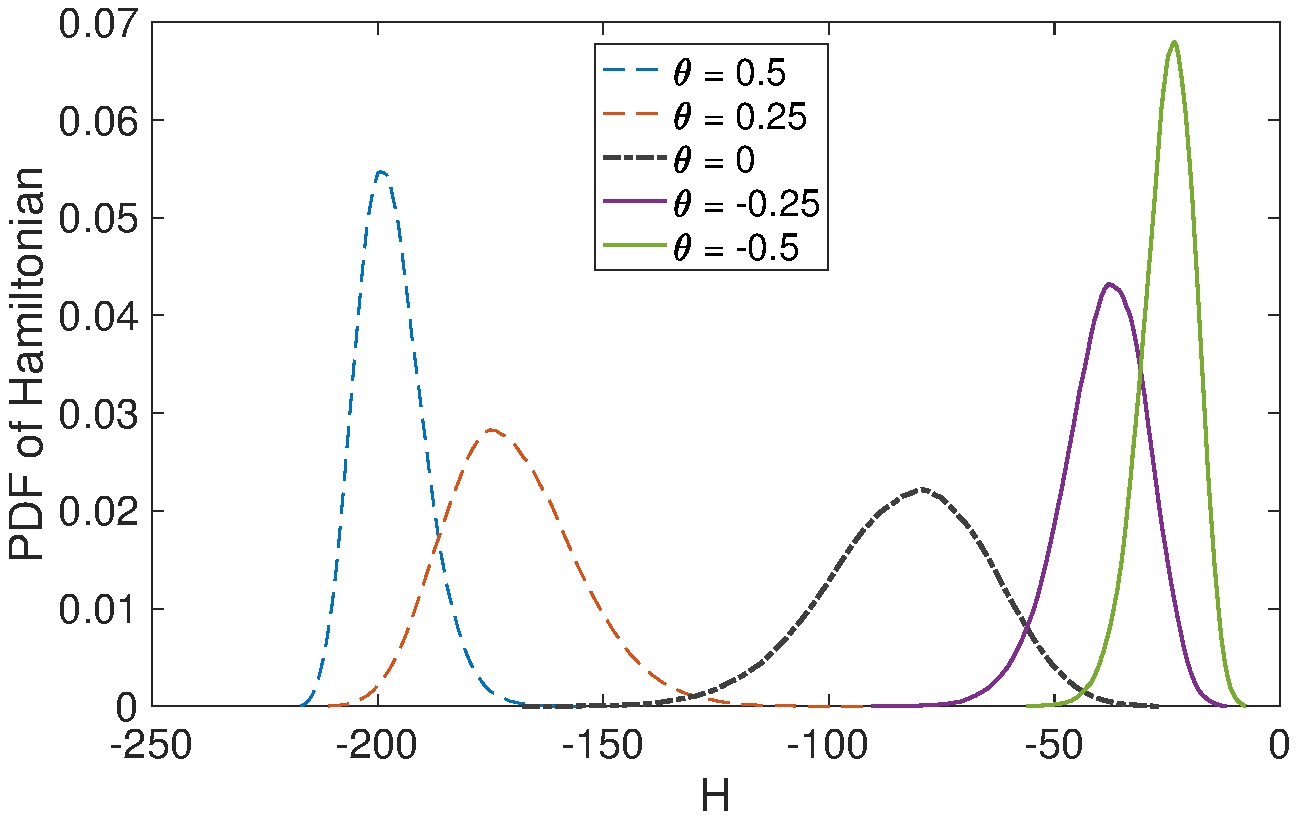
\includegraphics[scale=0.27]{./pdf0_hamil}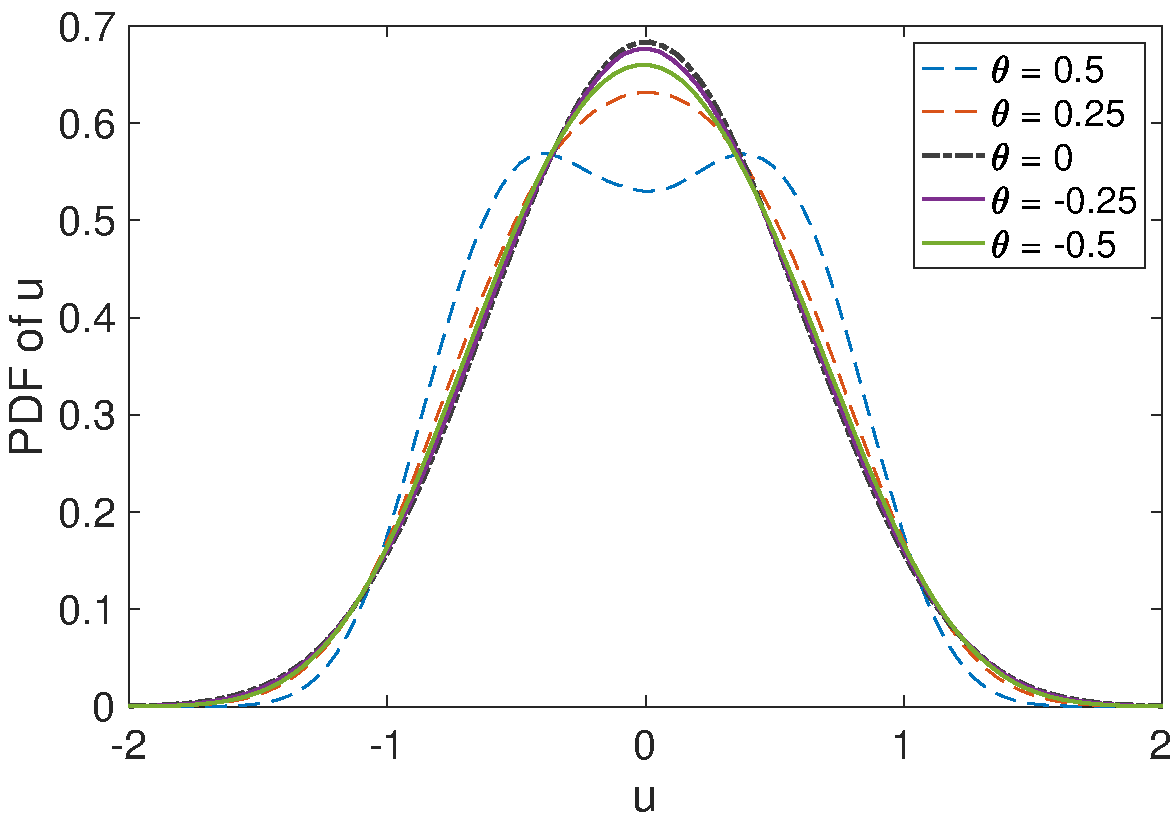
\includegraphics[scale=0.27]{./pdf0_u}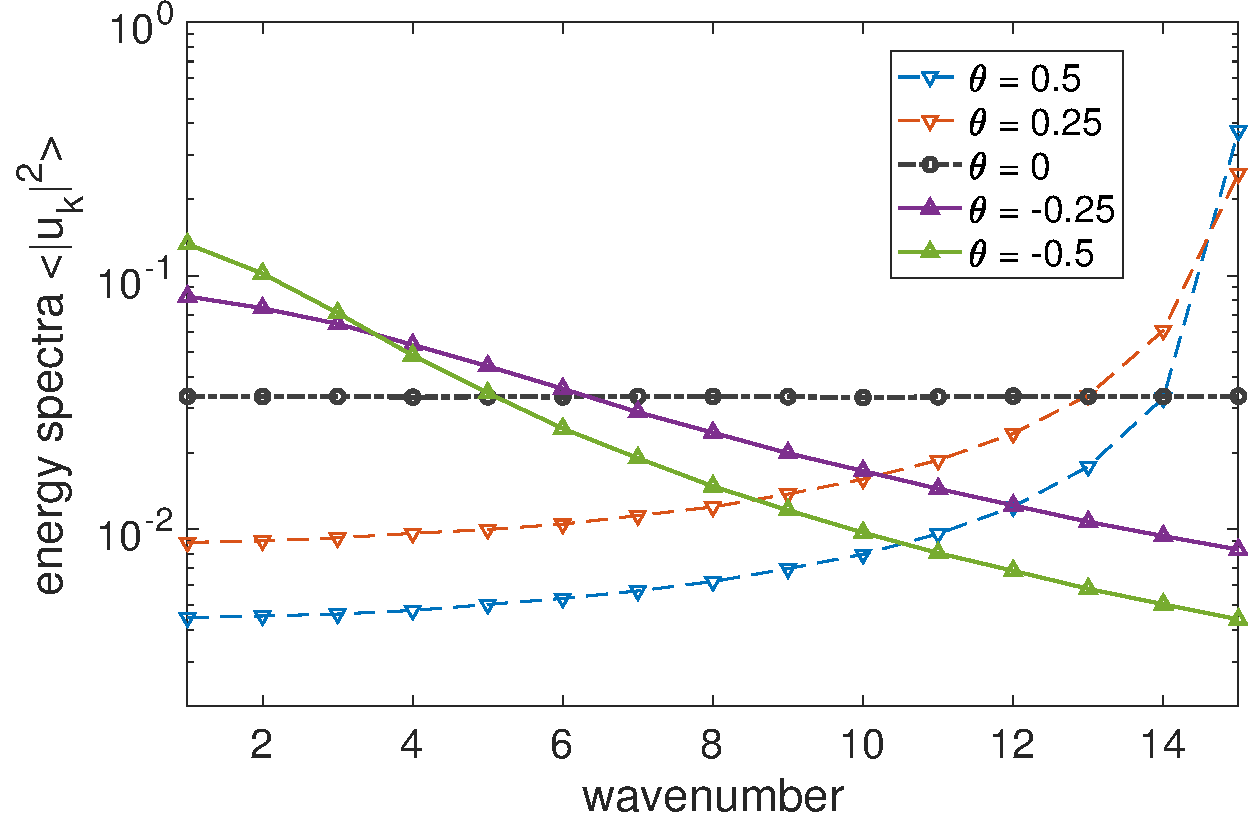
\includegraphics[scale=0.27]{./spec0}
\par\end{centering}
\caption{Statistics generated from the Gibbs invariant measures with different
inverse temperatures $\theta$ and $D_{0}=1$. Positive values of
$\theta$ are shown in dashed lines and negative values of $\theta$
in solid lines.\label{fig:Test-distributions}}
\end{figure}

\subsection{Computing downstream parameter from the statistical matching}

In the second step, we need to enforce the the statistical matching
condition [\ref{eq:matching}] to discover the corresponding downstream
inverse temperature $\theta^{+}$. For the efficiency of the method
in finding the optimal value of $\theta_{*}^{+}$, we use a secant
method by solving a nonlinear equation following the algorithm:
%\addtocounter{algorithm}{1}
\begin{algorithm}[H]
\caption{Recovering the downstream inverse temperature
$\theta^{+}$ from the statistical matching condition}\label{alg:Recovering}
%\begin{itemize}
\begin{algorithmic}[1]
\State Pick up the upstream value of $\theta^{-}$ and compute the expectation
under incoming flow Gibbs measure $\left\langle H_{\Lambda}^{+}\right\rangle _{\mathcal{G}_{\theta^{-}}}$;
\State Define a function of $\theta^{+}$ as the difference of the upstream
and downstream expectations, $F\left(\theta^{+}\right)=\left\langle H_{\Lambda}^{+}\right\rangle _{\mathcal{G}_{\theta^{+}}}-\left\langle H_{\Lambda}^{+}\right\rangle _{\mathcal{G}_{\theta^{-}}}$;
\State Find the solution of $F\left(\theta^{+}\right)=0$ using the secant
method, so that the optimal downstream value $\theta_{*}^{+}$ is
found.
%\end{itemize}
\end{algorithmic}
\end{algorithm}

In addition, to remove stiffness with large values of $L_0$ and $E_0$, we introduce the normalized parameter $\tilde{\theta}=L_{0}^{-3/2}\theta$ so that $\mathcal{G}_{\tilde{\theta}}\sim\exp\left(-\tilde{\theta}\left[E_{0}^{1/2}D_0^{-3/2}H_{3}-L_{0}^{-3/2}D_0^{1/2}H_{2}\right]\right)$. In the numerical computations, we tune the parameter $\tilde{\theta}$ instead for the matching condition. Using this modified secant method, it is found that the optimal value can be
usually reached after 2 to 5 iteration steps as long as the scheme
is guaranteed non-stiff. 

\subsubsection*{Numerical comparison of the matching results}

The solid black lines in Figure \ref{fig:Confirmation} plot the downstream
skewness $\kappa^{+}$ computed according to the matched downstream
$\theta^{+}$ as shown in Fig. 1 of the \textcolor{blue}{\emph{main text}}. Here as
a further comparison, the results with different total energy levels
$E_{0}$ starting from various various values of incoming $\theta^{-}$
are compared. Further, Table \ref{tab:Statistics-matching} compares
the incoming (with $\theta^{-}$) and outgoing (with $\theta^{+}$)
wave statistics using the parameters achieved from the statistical
matching condition. In the last two rows, the contributions of the
cubic term $H_{3}$ and quadratic term $H_{2}$ in the Hamiltonian
are compared in the incoming and outgoing flow statistics. It is found
that in the upstream statistics $\theta^{-}$, the quadratic part
$H_{2}$ is dominant, while in the downstream flow statistics, the
cubic part becomes important in the total Hamiltonian, implying stronger
non-Gaussian statistics.

As a further comparison, in the \textcolor{blue}{\emph{main text}} we also use the Gamma
distribution 
\[
\rho\left(u;k,\alpha\right)=\frac{e^{-k}\alpha^{-1}}{\Gamma\left(k\right)}\left(k+\alpha^{-1}u\right)^{k-1}e^{-\alpha^{-1}u},\quad\sigma^{2}=k\alpha^{2},\:\kappa_{3}=\frac{2}{\sqrt{k}},
\]
to fit the downstream state $u^{+}$ according to the measured skewness $\kappa_3$ and variance $\sigma^2$ for the parameters $\left(k,\alpha\right)$.
Table \ref{tab:Statistics-matching} also shows the fitting parameter
values according to the downstream statistics with $\theta^{+}$.
The Gamma fitting can also give an estimation for the kurtosis as
$\kappa_{4}=\frac{6}{k}+3$, which is shown to have good agreement
with the truth value $\kappa_4^{+}$ especially in the larger skewness
cases.

\begin{table}
\begin{centering}
\begin{tabular}{ccccc}
\toprule 
$\theta^{-}$ & $E_{0}=100$ & -0.5  & -0.3  & -0.1 \tabularnewline
\midrule
\midrule 
$\theta^{+}$ &  & -0.32  & -0.26  & -0.12 \tabularnewline
\midrule 
\multicolumn{2}{c}{$\left\langle H_{\Lambda}^{+}\right\rangle _{\theta^{-}}=\left\langle H_{\Lambda}^{+}\right\rangle _{\theta^{+}}$} & -9.57 & -15.72 & -28.17\tabularnewline
\midrule
\midrule 
\multirow{2}{*}{$\kappa_{3}$} & $\theta^{-}$ & 0.16 & 0.093 & 0.024\tabularnewline
\cmidrule{2-5} 
 & $\theta^{+}$ & 0.85 & 0.62 & 0.24\tabularnewline
\midrule
\multirow{1}{*}{$\kappa_{4}^{+}$} &  & 3.96 & 3.42 & 2.88\tabularnewline
\midrule
Gamma  & $\left(k,\alpha\right)$ & (5.5, 0.24) & (10.4, 0.18) & (68.0, 0.068)\tabularnewline
\cmidrule{2-5} 
fitting & $6/k+3$ & 4.08 & 3.58 & 3.08\tabularnewline
\midrule
\midrule 
\multirow{2}{*}{$\left\langle \tilde{H}_{3}\right\rangle _{\theta}$} & $\theta^{-}$ & 0.31 & 0.17 & 0.043\tabularnewline
\cmidrule{2-5} 
 & $\theta^{+}$ & 13.64 & 9.92 & 3.85\tabularnewline
\midrule 
\multirow{2}{*}{$\left\langle \tilde{H}_{2}\right\rangle _{\theta}$} & $\theta^{-}$ & 24.85 & 35.09 & 58.25\tabularnewline
\cmidrule{2-5} 
 & $\theta^{+}$ & 23.38 & 25.73 & 32.58\tabularnewline
\bottomrule
\end{tabular}
\par\end{centering}
\caption{Statistics computed from incoming and outgoing flow Gibbs measures
with $E_{0}=100$. The skewness $\kappa_{3}$ and kurtosis $\kappa_{4}$
predicted from the Gibbs measures with different $\theta^{-}$ are
compared. The outgoing statistics are compared with the Gamma function
fitting with parameter $\left(k,\alpha\right)$ and the corresponding
kurtosis $\kappa_{4}=6/k+3$. The expected values of the cubic and
quadratic terms in the Hamiltonian, $\tilde{H}_{3}=E_{0}^{1/2}L_{0}^{-3/2}D_{\pm}^{-3/2}\frac{1}{6}\int u^{3}$,
and $\tilde{H}_{2}=L_{0}^{-3}D_{\pm}^{1/2}\frac{1}{2}\int u_{x}^{2}$
are also compared.\label{tab:Statistics-matching}}
\end{table}

\subsubsection*{An explicit formula from the statistical matching condition}

In complementary to the \textcolor{blue}{\emph{main text}}, we offer a more detailed
derivation about the statistical link between the upstream and downstream
wave slope energy and the skewness. The statistical matching condition
with the downstream Hamiltonian can be written as
\[
\left\langle H_{\Lambda}^{+}\right\rangle _{\mu-}=\left\langle H_{\Lambda}^{+}\right\rangle _{\mu+},\;H_{\Lambda}^{+}=E_{0}^{1/2}L_{0}^{-3/2}D_{+}^{-3/2}H_{3}-L_{0}^{-3}D_{+}^{1/2}H_{2}.
\]
In general, we can have the expected value of $H_{3}$ and $H_{2}$
about any probability measure $\mu$ as
\[
\left\langle H_{3}\right\rangle _{\mu}=\frac{1}{6}\int_{0}^{2\pi}\left\langle u^{3}\right\rangle _{\mu-}dx=\frac{2\pi}{6J}\sum_{j=1}^{J}\left\langle u_{j}^{3}\right\rangle _{\mu},\;\left\langle H_{2}\right\rangle _{\mu}=\frac{1}{2}\int_{0}^{2\pi}\left\langle \left(u_{x}\right)^{2}\right\rangle _{\mu}dx=\frac{2\pi}{2}\sum_{\left|k\right|=1}^{\Lambda}k^{2}\left\langle \left|\hat{u}_{k}\right|^{2}\right\rangle _{\mu}.
\]
Above the quadratic term $H_{2}$ characterizes the \emph{slopes of
the surface waves}, $u_{x}$, in the incoming and outgoing flows.
Beside, the skewness the state variable $u$ at one grid point is
defined as the ratio between the third and second moments (note that
in the homogeneous model setup, we always have zero mean in the state
variable $\left\langle u\right\rangle \equiv0$)
\[
\kappa_{3}=\frac{\left\langle u_{j}^{3}\right\rangle _{\mu}}{\left\langle u_{j}^{2}\right\rangle _{\mu}^{\frac{3}{2}}},\quad\frac{1}{2}\int_{0}^{2\pi}\left\langle u^{2}\right\rangle _{\mu}dx=\frac{2\pi}{2J}\sum_{j=1}^{J}\left\langle u_{j}^{2}\right\rangle _{\mu}=1.
\]
Above the total energy of the system is normalized to one in the computations.
Now we use the two assumptions introduced in the main text:
\begin{itemize}
\item The upstream equilibrium measure $\mu_{-}$ has a near-Gaussian distribution,
so that the third moments in the cubic term stay in a small value
\[
\left\langle H_{3}\right\rangle _{\mu-}=\frac{1}{6}\int_{0}^{2\pi}\left\langle u^{3}\right\rangle _{\mu-}dx=\epsilon;
\]
\item The downstream equilibrium measure $\mu_{+}$ is homogeneous at each
physical grid point, so that the second and third moments are invariant
at each grid point
\[
\left\langle u_{j}^{2}\right\rangle _{\mu+}=\sigma^{2}=\pi^{-1},\quad\left\langle u_{j}^{3}\right\rangle _{\mu+}=\sigma^{3}\kappa_{3}=\pi^{-\frac{3}{2}}\kappa_{3}.
\]
\end{itemize}
With the homogeneous assumption above, the downstream cubic term can
be simplified as
\[
\left\langle H_{3}\right\rangle _{\mu+}=\frac{\pi}{3J}\sum_{j=1}^{J}\left\langle u_{j}^{3}\right\rangle _{\mu+}=\frac{1}{3}\pi^{-\frac{1}{2}}\kappa_{3}.
\]
With the above assumptions, the above statistical matching condition
can be simplified as
\begin{align*}
E_{0}^{1/2}L_{0}^{-3/2}D_{+}^{-3/2}\epsilon & -L_{0}^{-3}D_{+}^{1/2}\left\langle H_{2}\right\rangle _{\mu-}=E_{0}^{1/2}L_{0}^{-3/2}D_{+}^{-3/2}\left\langle H_{3}\right\rangle _{\mu+}-L_{0}^{-3}D_{+}^{1/2}\left\langle H_{2}\right\rangle _{\mu+}\\
\Rightarrow\; & E_{0}^{1/2}L_{0}^{-3/2}D_{+}^{-3/2}\epsilon+\pi L_{0}^{-3}D_{+}^{1/2}\sum_{1\leq\left|k\right|\leq\Lambda}k^{2}\left(r_{k}^{+}-r_{k}^{-}\right)=\frac{1}{3}\pi^{-1/2}E_{0}^{1/2}L_{0}^{-3/2}D_{+}^{-3/2}\kappa_{3},
\end{align*}
with $r_{k}^{-}=\left\langle \left|\hat{u}_{k}\right|^{2}\right\rangle _{\mu-}$
the variance in upstream statistics and $r_{k}^{+}=\left\langle \left|\hat{u}_{k}\right|^{2}\right\rangle _{\mu+}$
the statistics from downstream statistics. Therefore we can estimate
the skewness of the state variable $u$ from the energy spectra in
inflow and outflow statistics
\begin{equation}
\kappa_{3}^{+}=3\pi^{\frac{3}{2}}L_{0}^{-\frac{3}{2}}E_{0}^{-\frac{1}{2}}D_{+}^{2}\sum_{1\leq\left|k\right|\leq\Lambda}k^{2}\left(r_{k}^{+}-r_{k}^{-}\right)+3\pi^{\frac{1}{2}}\epsilon.\label{eq:skewness}
\end{equation}
With further assumption that the incoming flow gets zero third moment,
then the skewness above can be calculated by
\[
\kappa_{3}^{+}=C\sum_{1\leq\left|k\right|\leq\Lambda}k^{2}\left(r_{k}^{+}-r_{k}^{-}\right),\;C=3\pi^{\frac{3}{2}}L_{0}^{-\frac{3}{2}}E_{0}^{-\frac{1}{2}}D_{+}^{2},
\]
with the coefficient $C$ depending on the model setup. Especially,
we can see that a positive skewness can be generated from $r_{k}^{+}>r_{k}^{-}$
in small scale modes and $r_{k}^{+}<r_{k}^{-}$ in large scales. The
total energy of the system is always normalized to unit, $\pi\sum r_{k}^{+}=\pi\sum r_{k}^{-}=1$. 

Notice that in [\ref{eq:skewness}], the spectral difference between
the incoming and outgoing flows
\[
\sum_{1\leq\left|k\right|\leq\Lambda}k^{2}\left(r_{k}^{+}-r_{k}^{-}\right)=\frac{1}{2\pi}\int_{0}^{2\pi}\left[\left\langle \left(u_{x}\right)^{2}\right\rangle _{\mu+}-\left\langle \left(u_{x}\right)^{2}\right\rangle _{\mu-}\right]dx,
\]
calibrates the statistics in the `waves slopes', $u_{x}$, before
and after the depth change. Therefore, the skewness in the surface
wave displacement statistics is connected with the waves slopes between
the incoming and outgoing waves. This is consistent with the physical
understanding in the flow field, since a stronger slope in the waves
always implies the larger skewness in the disturbance.

In Figure \ref{fig:Confirmation}, we compare the accuracy of the
theoretical estimation derived above using numerical tests. In the
regime with small incoming inverse temperature $\theta^{-}$, the
theoretical formula in [\ref{eq:skewness}] offers quite accurate
approximation of the third-order skewness using only information from
the second-order moments of the wave-slope spectrum. When $\theta^{-}$
grows larger in amplitude, the error without the incoming flow correction
becomes large. The improvement is obvious by adding the correction
from the incoming wave skewness $\kappa^{-}$. However, for the statistical
matching condition, there exists a maximum amplitude threshold of
$\theta^{-}$ for the matching to be valid (so that $\left\langle H^{-}\right\rangle $
stays negative). The maximum threshold value of $\theta^{-}$ is marked
by the dashed vertical line.

\begin{figure}
\begin{centering}
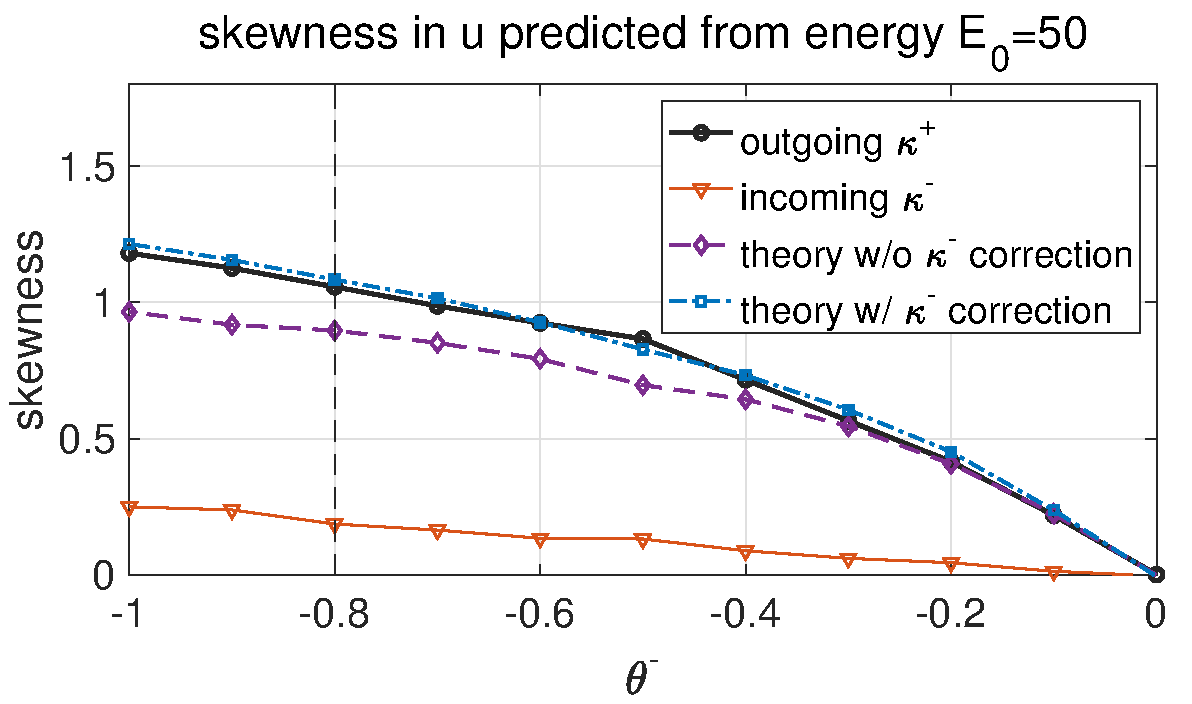
\includegraphics[scale=0.28]{./matchTheory_E50}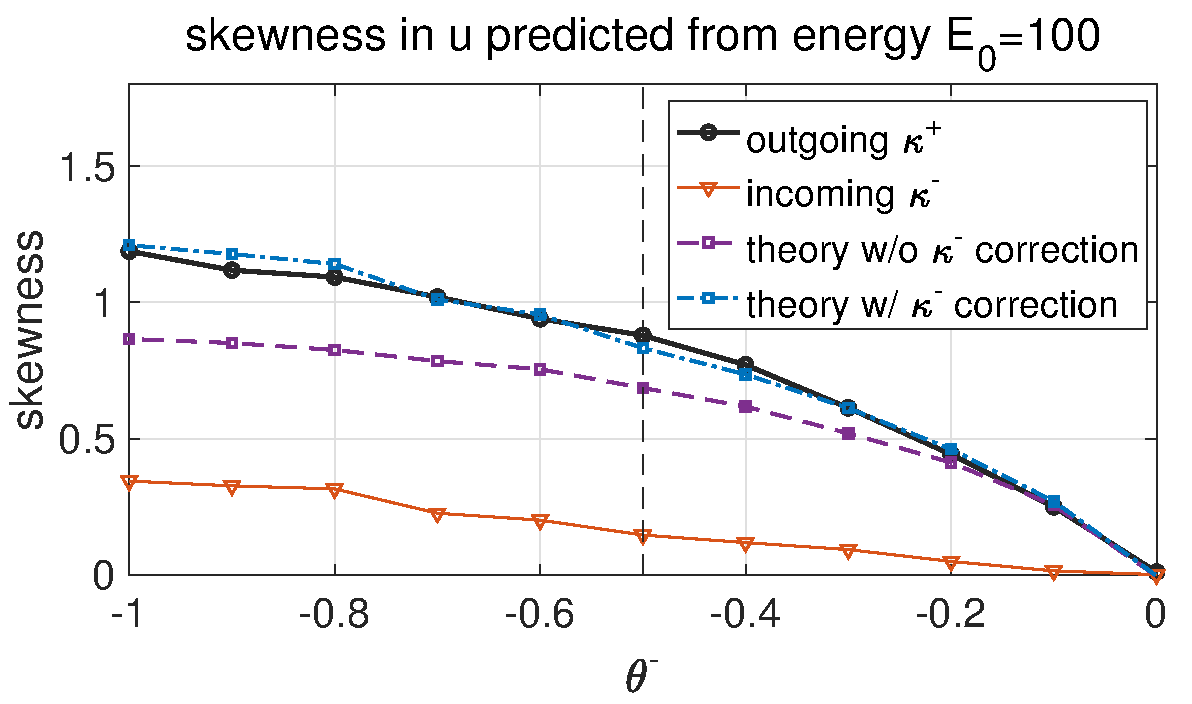
\includegraphics[scale=0.28]{./matchTheory_E100}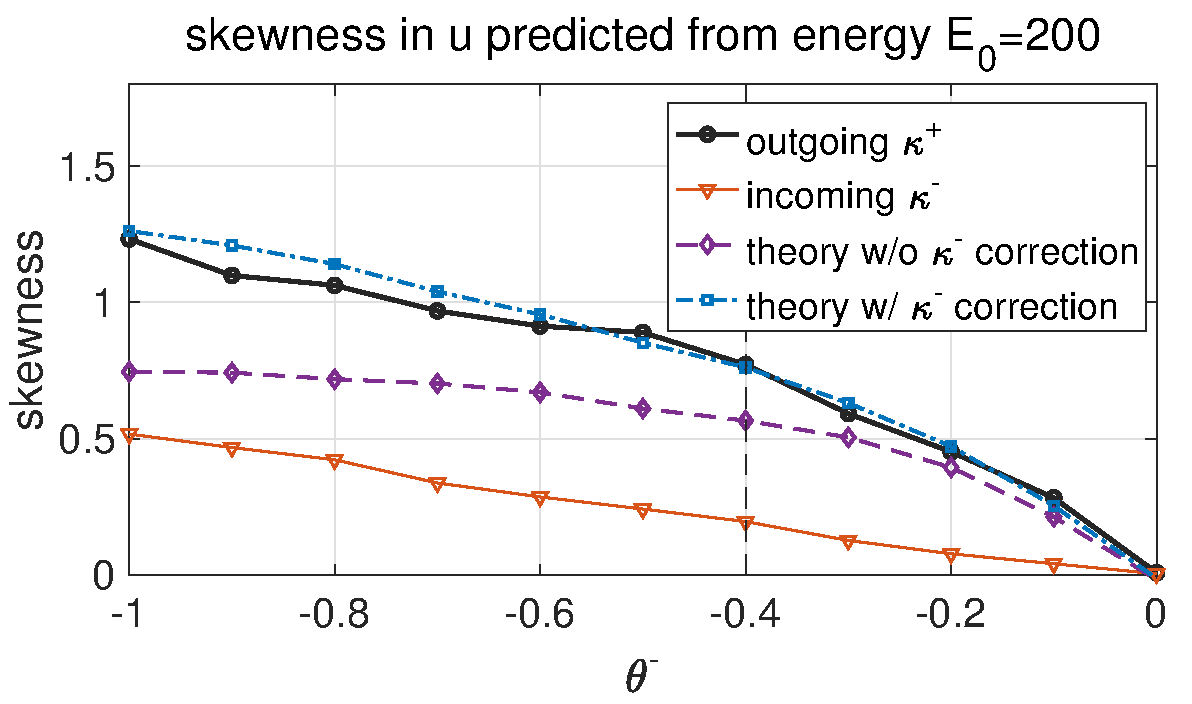
\includegraphics[scale=0.28]{./matchTheory_E200}
\par\end{centering}
\caption{Confirmation of the theoretical approximation of the skewness in the
state $u$ using energy in the wave slope $u_{x}$. The results with
and without the incoming flow skewness correction $\kappa_{3}^{-}$
are compared. The vertical line marks the value where the statistical
matching condition is valid.\label{fig:Confirmation} }
\end{figure}

\section{Symplectic scheme for direct numerical simulations of the TKdV equation}

Here we summarize the direct numerical methods used for the validation
of the statistical theory in the \textcolor{blue}{\emph{main text}}. In general, the
strategy by using direct numerical simulations to confirm the anomalous
statistics follows the steps:
\begin{enumerate}
\item Generate samples from the incoming equilibrium distribution $\mu_{\infty}^{-}$
according to Algorithm \ref{alg:Metropolis-Hastings} for the incoming
waves. The model parameters $\left(E_{0},L_{0},\Lambda\right)$ are
determined from the experimental measurements and statistics in the
incoming flow;
\item Compute the expectation of the outflow Hamiltonian, $\left\langle H_{\Lambda}^{+}\right\rangle _{\mu_{\infty}^{-}}$,
under the chosen incoming Gibbs measure $\mu_{\infty}^{-}=\mathcal{G}_{\theta^{-}}$;
\item The outgoing flow statistics can be predicted by both the equilibrium
statistical mechanism and the direction model simulations. 
\begin{enumerate}
\item Equilibrium statistical mechanism: find the optimal outgoing flow
parameter $\theta_{*}^{+}$ from matching the expectation in [\ref{eq:matching}]
with the inflow value according to Algorithm \ref{alg:Recovering}.
Then the new equilibrium distribution $\mu_{\infty}^{+}$ after the
abrupt depth change can be sampled using the same method;
\item Direct model simulations: run the dynamical model [\ref{eq:KdV_simu}]
with outflow depth $D_{+}<1$ starting from the state sampled from
the inflow distribution $\mathcal{G}_{\theta^{-}}$. The outgoing
flow statistics can be captured by the solution from the direction
simulations. 
\end{enumerate}
\end{enumerate}
Above we proposed two approaches to predict the statistics in the
downstream wave disturbance. The equilibrium statistical mechanism
is an easy way to confirm the matching condition and get the equilibrium
distribution in far-field long-time limit. On the other hand, the
direct simulations of the dynamical model can offer estimates about
the transient statistics before the far-field equilibrium state is
reached. These two approaches can be used to confirm each other in
the numerical results.

\subsection{Conservation of energy and Hamiltonian form the symplectic scheme}

For running the direct numerical simulations of the TKdV equations,
a proper symplectic integrator is necessary to guarantee the conservation
of the Hamiltonian and energy in time. As emphasized in the \textcolor{blue}{\emph{main
text}}, the conservation property plays a central role in the statistical
matching and the final equilibrium measure, otherwise the non-symplectic
schemes introduce high numerical dissipations. The symplectic scheme
used here for the time integration of equation [\ref{eq:KdV_simu}]
is the 4th-order midpoint method \cite{mclachlan1993symplectic}.
Let $\mathbf{u}^{n}$ be the solution at time $t_{n}$ and $\mathbf{u}^{n+1}$
be the solution at next time step $t_{n+1}=t_{n}+\Delta t$, and $\mathbf{F}$the
discretized operator for the spectral modes. The midpoint method has
two intermediate stages and the auxiliary vectors $\mathbf{y}_{1},\mathbf{y}_{2}$
\[
\begin{aligned}\mathbf{y}_{1}-\mathbf{u}^{n} & =w_{1}\Delta t\mathbf{F}\left(\frac{1}{2}\left[\mathbf{y}_{1}+\mathbf{u}^{n}\right]\right),\\
\mathbf{y}_{2}-\mathbf{y}_{1} & =w_{2}\Delta t\mathbf{F}\left(\frac{1}{2}\left[\mathbf{y}_{2}+\mathbf{y}_{1}\right]\right),\\
\mathbf{u}^{n+1}-\mathbf{y}_{2} & =w_{3}\Delta t\mathbf{F}\left(\frac{1}{2}\left[\mathbf{u}^{n+1}+\mathbf{y}_{2}\right]\right),
\end{aligned}
\]
with the time increments $w_{1}=\left(2+2^{1/3}+2^{-1/3}\right)/3$,
$w_{2}=1-2w_{1}$, and $w_{3}=w_{1}$. Then the PDFs can be counted
from the solution $u_{\Lambda}\left(t\right)$, and the statistical
expectations can be calculated by averaging along the trajectory
\[
\left\langle F\left(u_{\Lambda}\right)\right\rangle _{\mu}=\frac{1}{T}\int_{t_{0}}^{t_{0}+T}F\left(u_{\Lambda}\left(t\right)\right)dt,
\]
given ergodicity in the solution with $u_{\Lambda}\left(t_{0}\right)$
already reaching the stationary state.

We compare the statistical spectra from the direct Monte Carlo model
simulation with the prediction from the equilibrium statistical mechanism
in Figure \ref{fig:Comparison-spec }. The flow energy spectra computed
both from the direct TKdV model simulations and from the Gibbs invariant
measure in the equilibrium statistical mechanism are compared. Starting
from two different $\theta^{-}$ initial states, the direct model
simulations offer the final equilibrium energy spectrum in a cimparable
decaying structure as predicted from the Gibbs measure and statistical
matching condition. This first comparison offers the consistency in
these two distinct approaches.

\begin{figure}
\begin{centering}
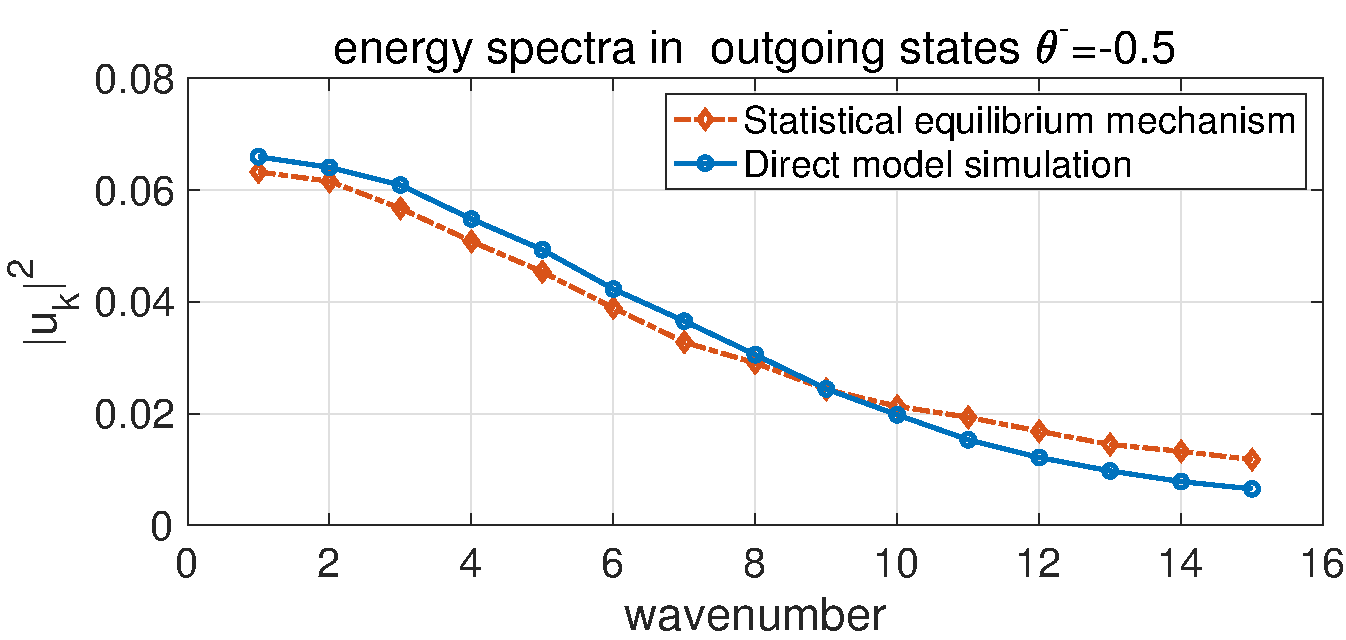
\includegraphics[scale=0.32]{./specEqui_th05}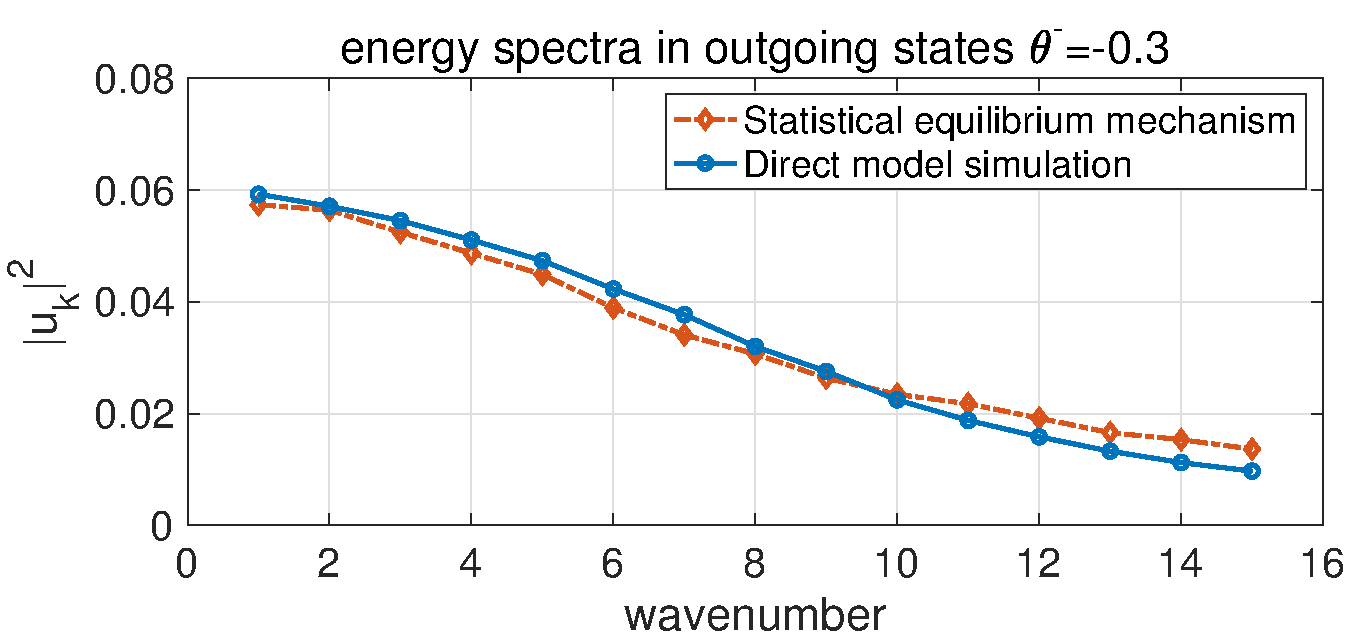
\includegraphics[scale=0.32]{./specEqui_th03}
\par\end{centering}
\caption{Comparison of the energy spectra computed from directly running the numerical 
model and the energy spectra predicted from the
Gibbs invariant measure in equilibrium statistical mechanism. The
model simulations start with the Gibbs measure with different
incoming flow parameter $\theta^{-}$.\label{fig:Comparison-spec }}
\end{figure}

\subsection{Ergodicity and mixing properties in the TKdV solutions}

Ergodicity is another crucial feature that needs to be confirmed in
the TKdV equation solution. To achieve reasonable statistics
from averaging the model time solutions, it is important to make sure
that the solution is turbulent mixing. Following we display the
direct numerical simulation solutions from the TKdV equation using
initial states sampled from different inverse temperatures.

\subsubsection*{Mixing solutions starting from negative inverse temperature $\theta<0$}

In the \textcolor{blue}{\emph{main text}}, the results shown always use negative inverse
temperature. As shown from \cite{abramov2003hamiltonian,bajars2013weakly}
and Figure \ref{fig:Test-distributions} before, this is a reasonable
choice to generate a decaying energy spectrum. Here as a further illustration,
we show that the negative inverse temperature case also generates
fast mixing solutions to calculate reasonable statistical averages.

In Figure \ref{fig:Realization1} and \ref{fig:Realization2}, we
display the single trajectory solutions for both downstream $D_{+}=0.24$
and upstream $D_{-}=1$ flows. The initial state is taken from the
samples in Algorithm \ref{alg:Metropolis-Hastings} with a negative
initial temperature $\theta<0$. The other parameters are kept the
same as in the main text. On the left panel, the contour plot for
the time-series of $u_{\Lambda}$ is shown for the downstream and
upstream flows. Both cases display turbulent dynamics, while the downstream
solution with $D_{+}<0$ generates more rare events and stronger turbulence.

For more detailed comparison, the right panels show one slice of the
time-series of $u_{\Lambda}\left(x_{1}\right)$ at one physical location
as well as the first two Fourier modes, $\hat{u}_{1},\hat{u}_{2}$,
in the spectral domain. The rare events in the downstream solution
in Figure \ref{fig:Realization1} is obvious with high peaks representing
the generation of skewed PDFs in the positive direction. In comparison,
the upstream solution in Figure \ref{fig:Realization2} displays almost
symmetric values in positive and negative disturbances, implying near-Gaussian
statistics in the incoming flow. The mixing properties are characterized
by the autocorrelation and decorrelation time of the state variable.
The decorrelation time $T_{k}$ and absolute decorrelation time $T_{k}^{\mathrm{abs}}$
together with the autocorrelation function $\mathcal{R}_{k}$ in each
spectral mode are defined as
\[
T_{k}=\left|\int\mathcal{R}_{k}\left(t\right)dt\right|,\;T_{k}^{\mathrm{abs}}=\int\left|\mathcal{R}_{k}\left(t\right)\right|dt,\quad\mathcal{R}_{k}\left(t\right)=\left\langle \hat{u}_{k}\left(0\right)\hat{u}_{k}\left(t\right)^{*}\right\rangle /\left\langle \left|\hat{u}_{k}\right|^{2}\right\rangle .
\]
Decaying autocorrelations in both the physical state and the spectral
modes confirm the fast mixing and turbulent dynamics in both the tested
regimes used in the main text (though weaker in upstream). We can
observe the much faster time scales in the downstream flow in the
autocorrelation functions in the corresponding time-series. The longer
decorrelation times in the upstream flow indicate oscillating autocorrelations
for a long time.

\begin{figure}[h]
\begin{centering}
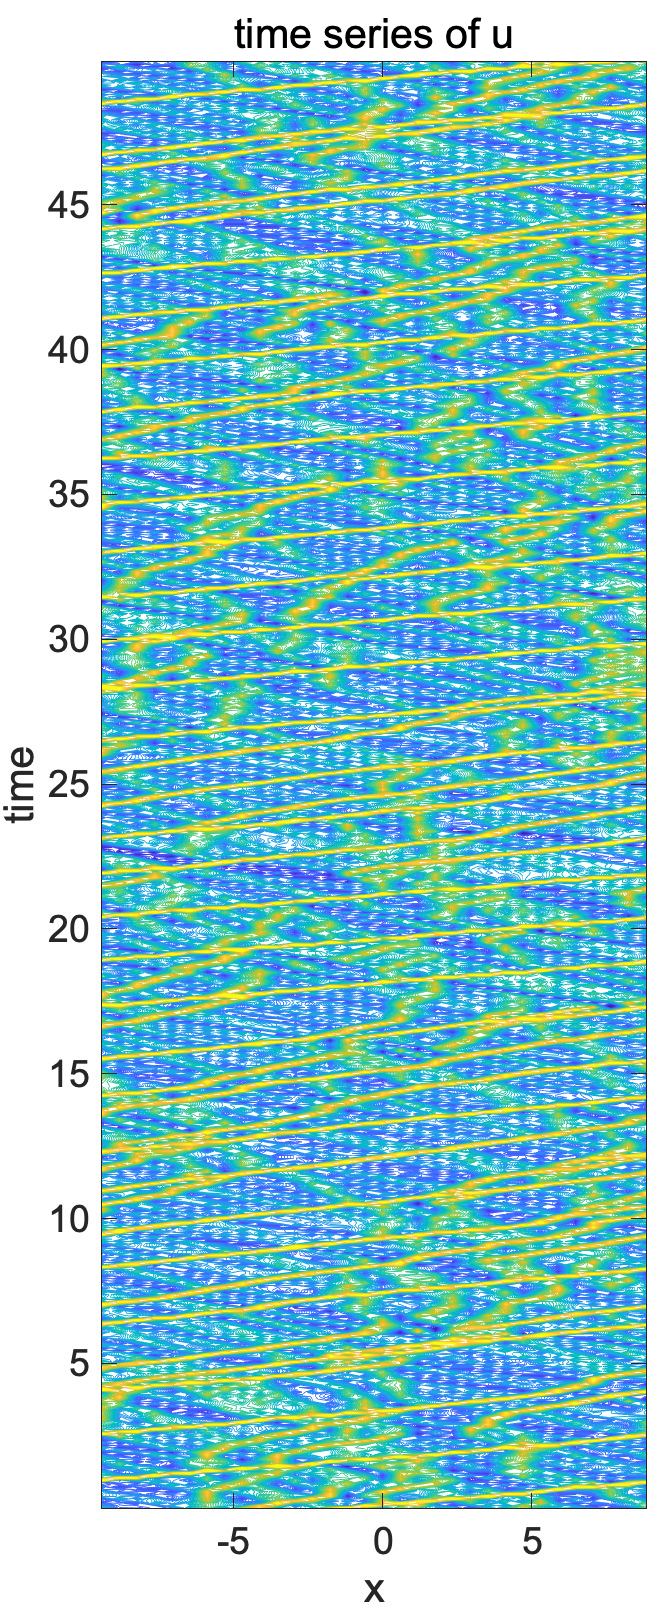
\includegraphics[scale=0.35]{./snap_J32L3D024E100}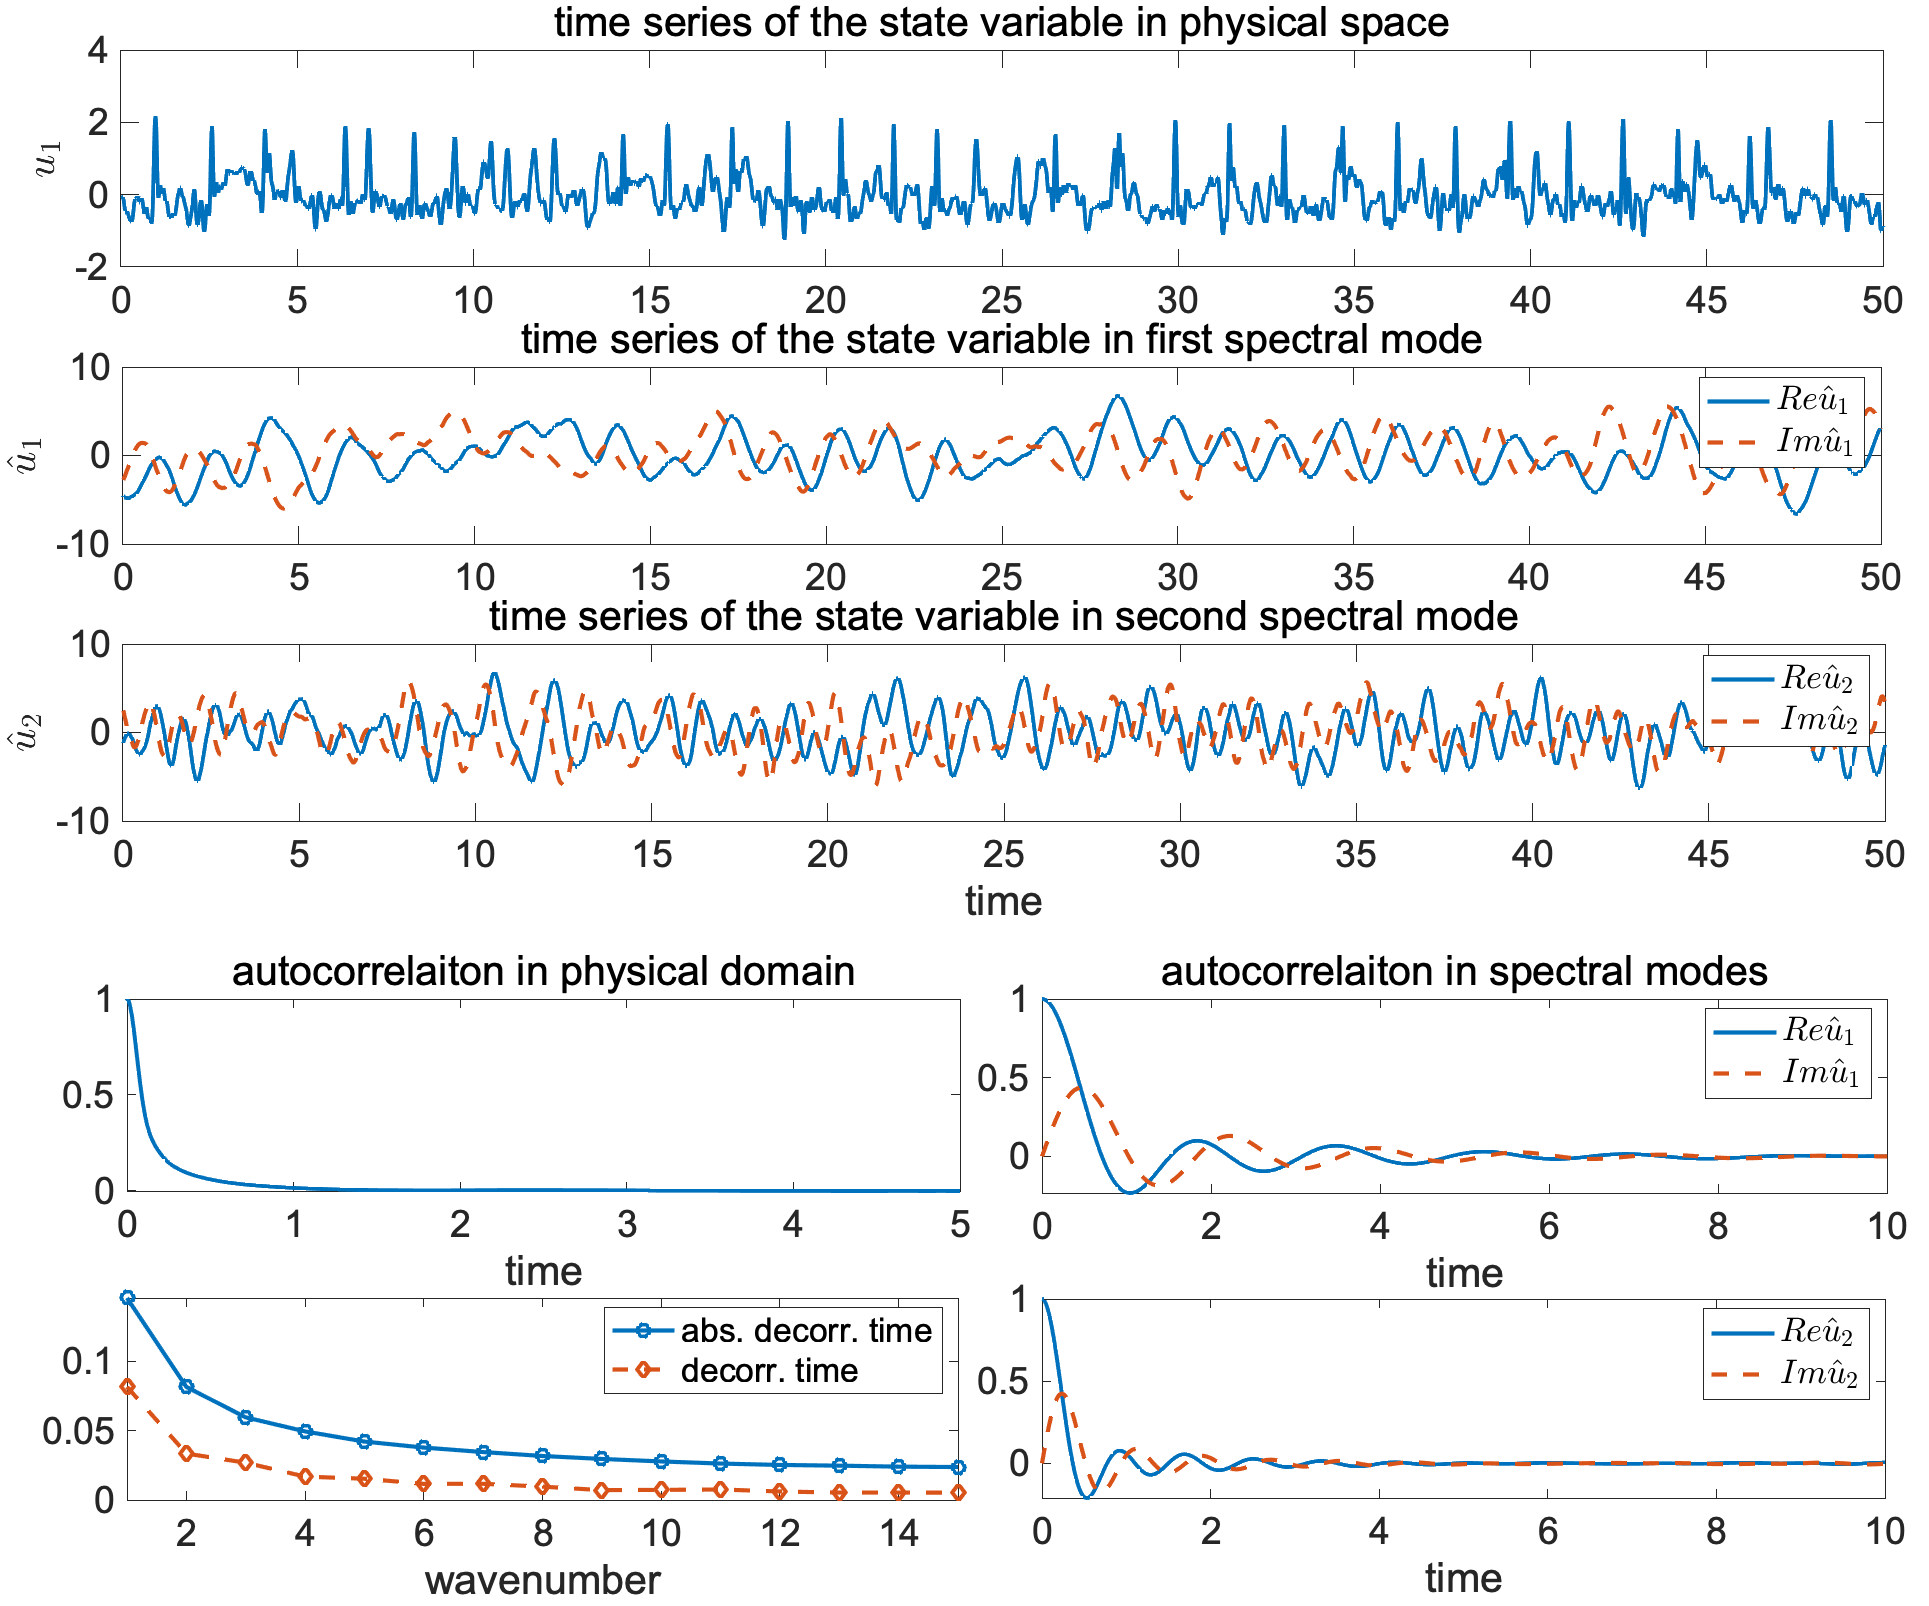
\includegraphics[scale=0.35]{./tseries1_J32L3D024E100}
\par\end{centering}
\caption{Realization of the downstream flow solution with $D_{0}=0.24$ and
initial state from samples with negative inverse temperature.\label{fig:Realization1}}

\end{figure}
\begin{figure}[h]
\begin{centering}
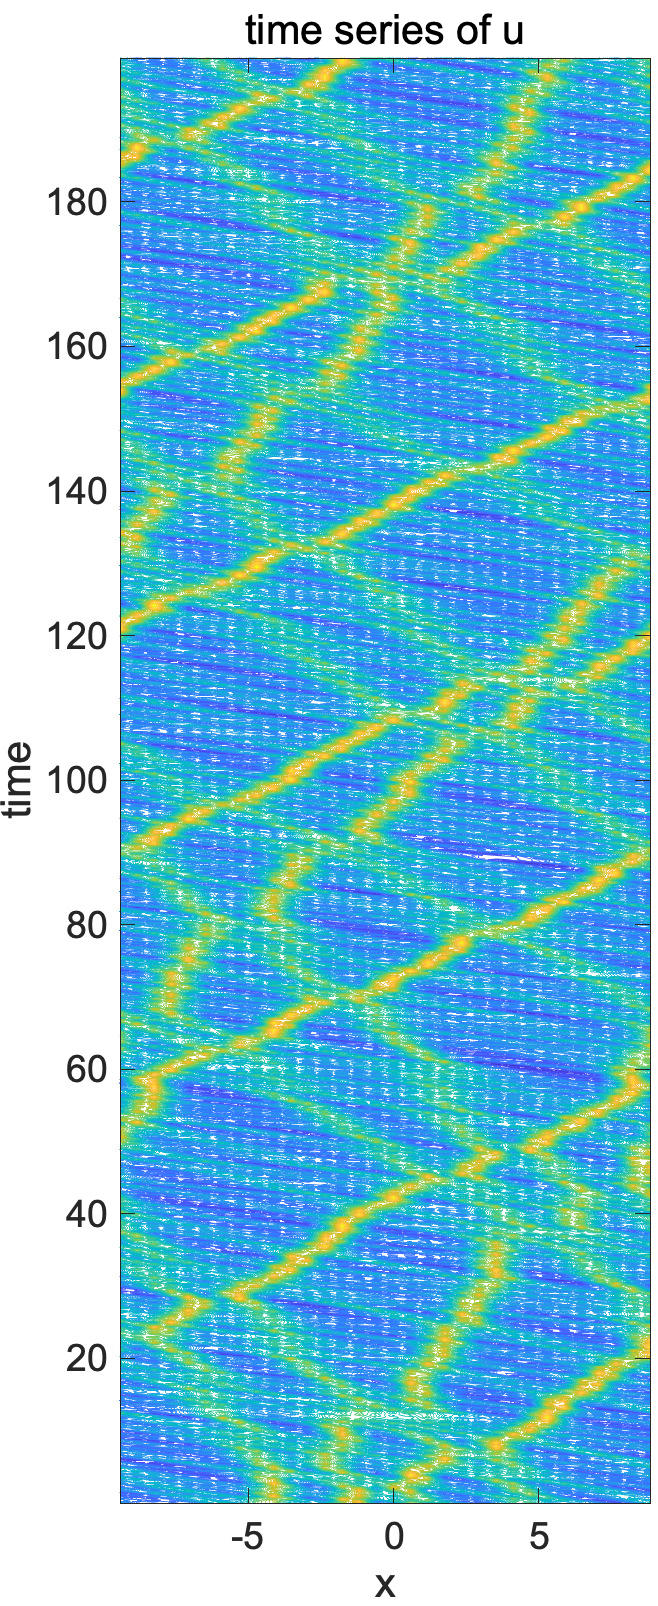
\includegraphics[scale=0.35]{./snap1_J32L3D1E100}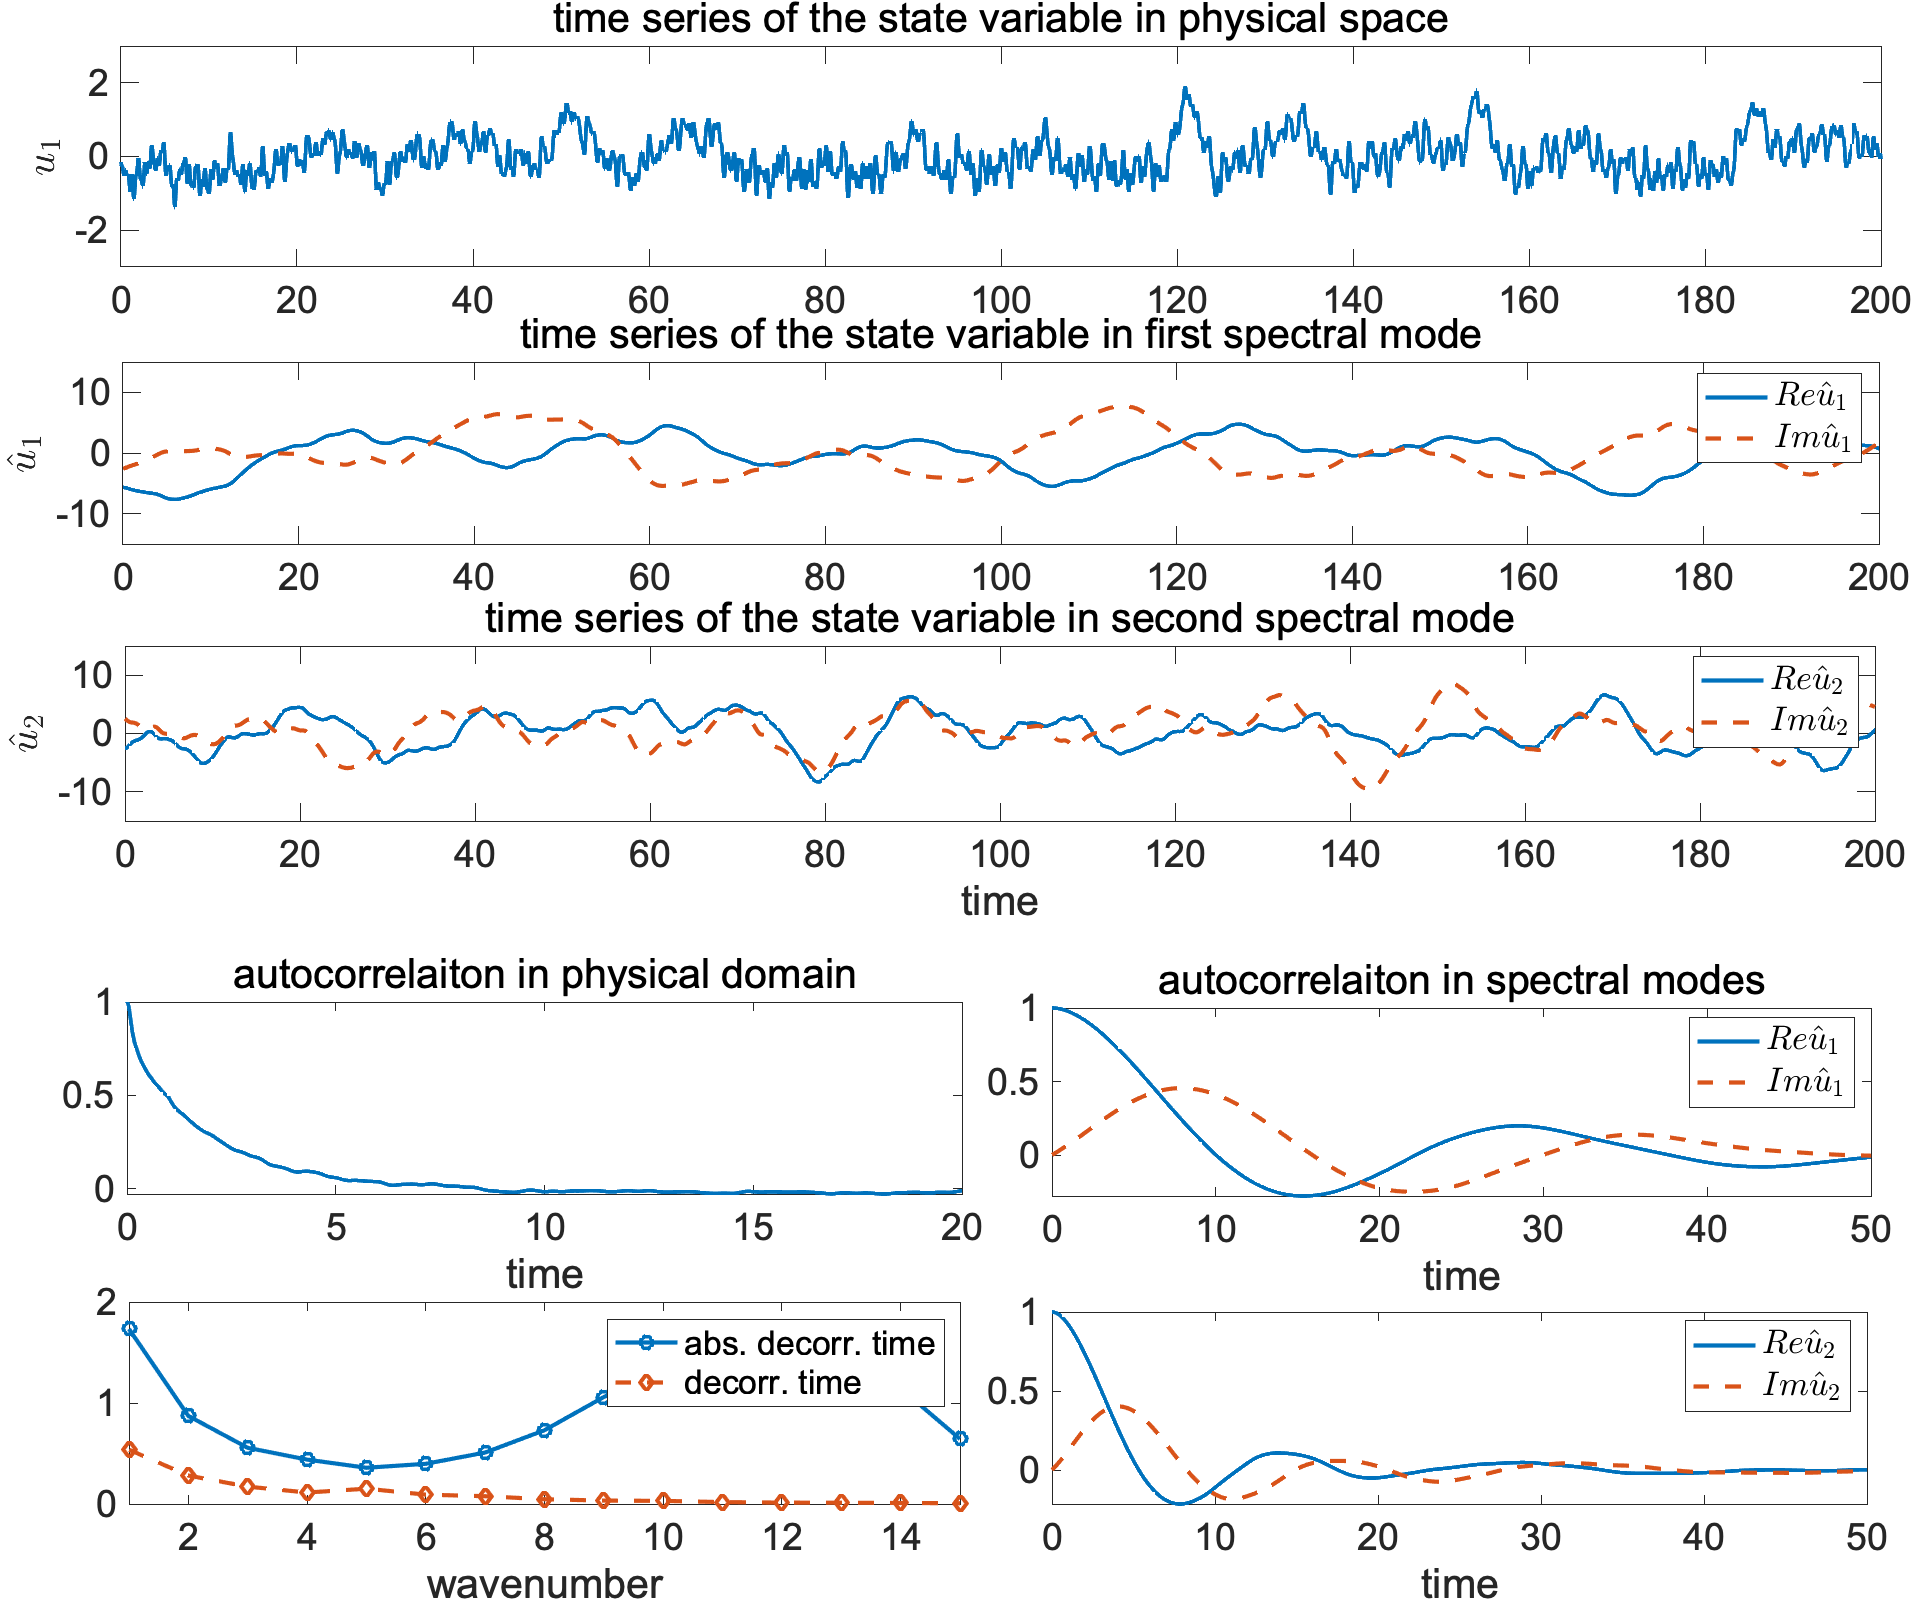
\includegraphics[scale=0.35]{./tseries1_J32L3D1E100}
\par\end{centering}
\caption{Realization of the upstream flow solution with $D_{0}=1$ and initial
state from samples with negative inverse temperature.\label{fig:Realization2}}
\end{figure}
As an additional comparison, we show the power spectra of the upstream
and downstream flows from the above test cases in Figure \ref{fig:Power-spectra}.
The power spectrum can be calculated by the Fourier transform of the
autocorrelation function
\[
S\left(\lambda\right)=\int_{-\infty}^{\infty}\mathcal{R}\left(\tau\right)e^{-i\lambda\tau}d\tau,
\]
which offers the characterization of the decay in power at each time
frequency. Again, consistent with the observations from experiments
\cite{bolles2018anomalous} and the numerics in the \textcolor{blue}{\emph{main text}},
the downstream power spectrum gets more energetic small time scales
at low frequency modes and a slower decay rate in the high frequency
modes compared with the upstream case. Also notice that the peak in
the incoming flow power spectrum is taken place at a much lower frequency.
This illustrates the slower mixing rate in the incoming flow state.

\begin{figure}[h]
\begin{centering}
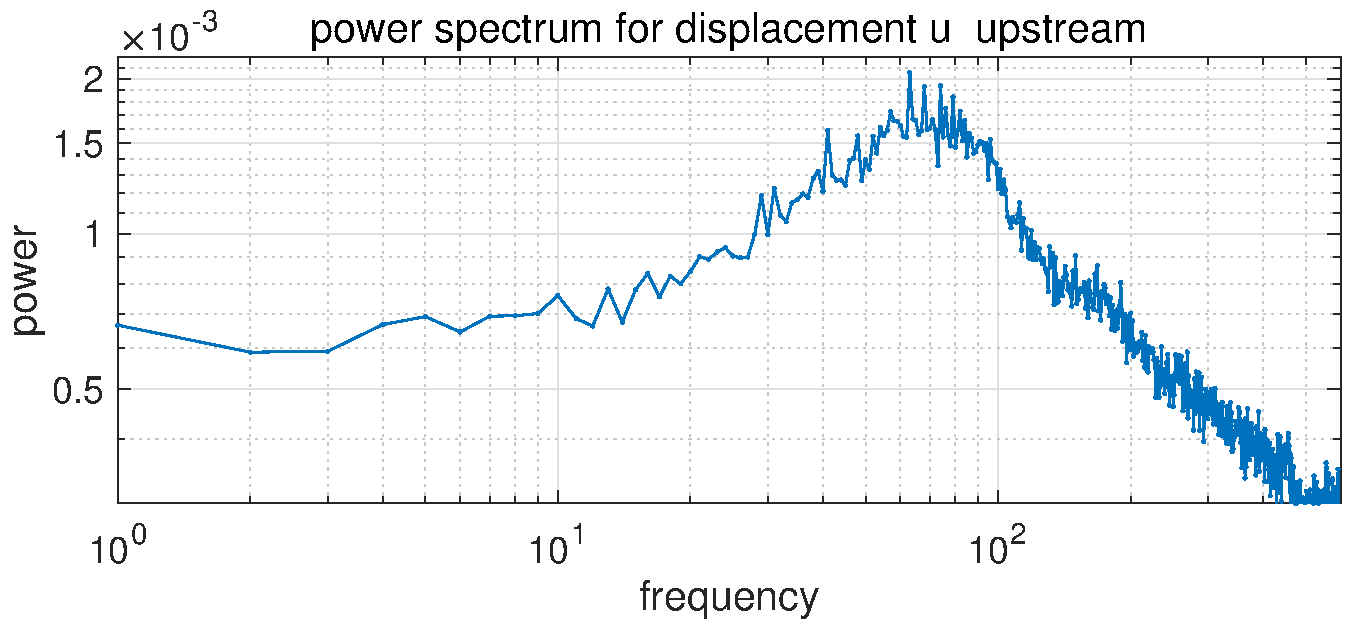
\includegraphics[scale=0.32]{./power_up}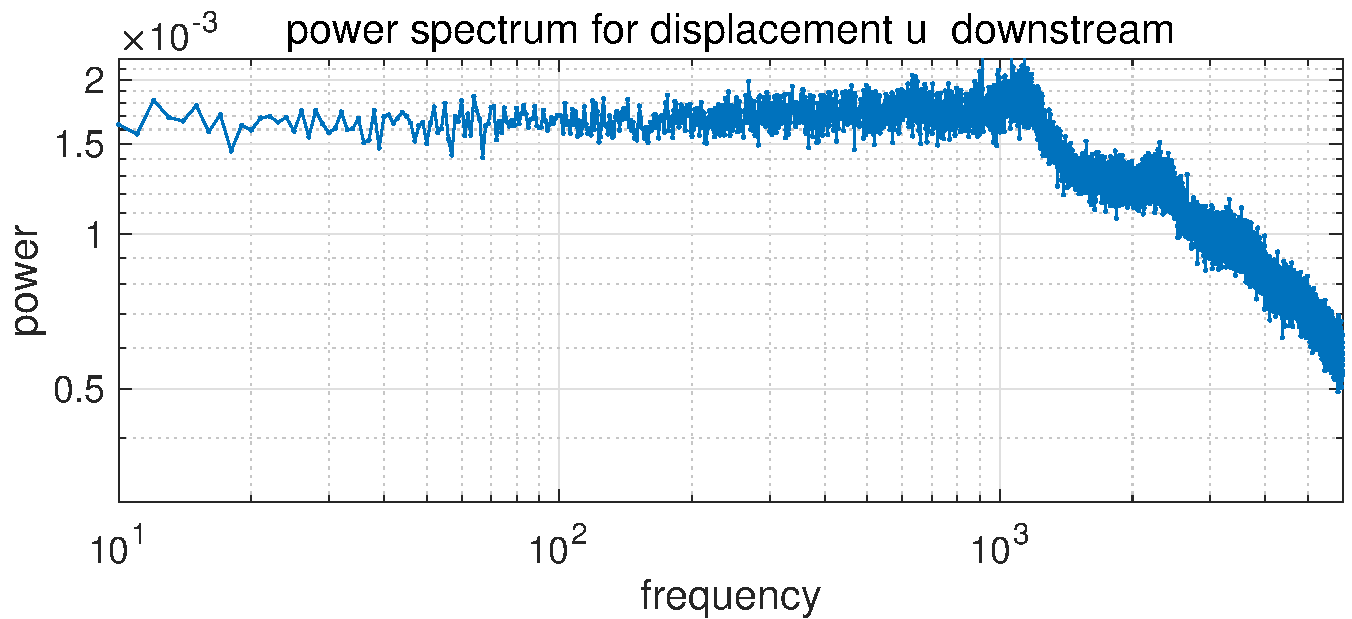
\includegraphics[scale=0.32]{./power_down}
\par\end{centering}
\caption{Power spectra of the upstream and downstream states $u_{\Lambda}$.\label{fig:Power-spectra}}

\end{figure}

\subsubsection*{Non-mixing solutions starting from positive inverse temperature $\theta>0$}

In comparison, we also compute the solution starting from an initial
state with a positive inverse temperature $\theta>0$. In contrast to
the previous case in Figure \ref{fig:Realization2}, the only difference
in the present case is the initial state taken from the samples in
an invariant measure with positive inverse temperature. Figure \ref{fig:Realization3}
displays the corresponding solution in this 
$\theta>0$ case. In contrast to the previous mixing solution with
negative inverse temperature, drastic difference performance is generated
due to only the change in the initial state. The solution is recurrent in time with interacting small scales. As a result, the solution
in stationary waves lacks the proper mixing property and the autocorrelation just
oscillates for an extremely long time.

Accordingly in the autocorrelation functions and decorrelation times,
the autocorrelation functions just keep oscillating and all the modes
get long absolute decorrelation time (the decorrelation time is small
due to the cancellation from the oscillations). This non-mixing feature
with positive temperature supports the conclusion in the main text
that this regime is not appropriate for correctly representing the
physical statistics in the experimental setups. This simple test further
confirms the unrealistic energy spectra in the positive temperature
case with increasing energy in the smaller scales shown in \cite{bajars2013weakly}
and Figure \ref{fig:Test-distributions}.

\begin{figure}[h]
\begin{centering}
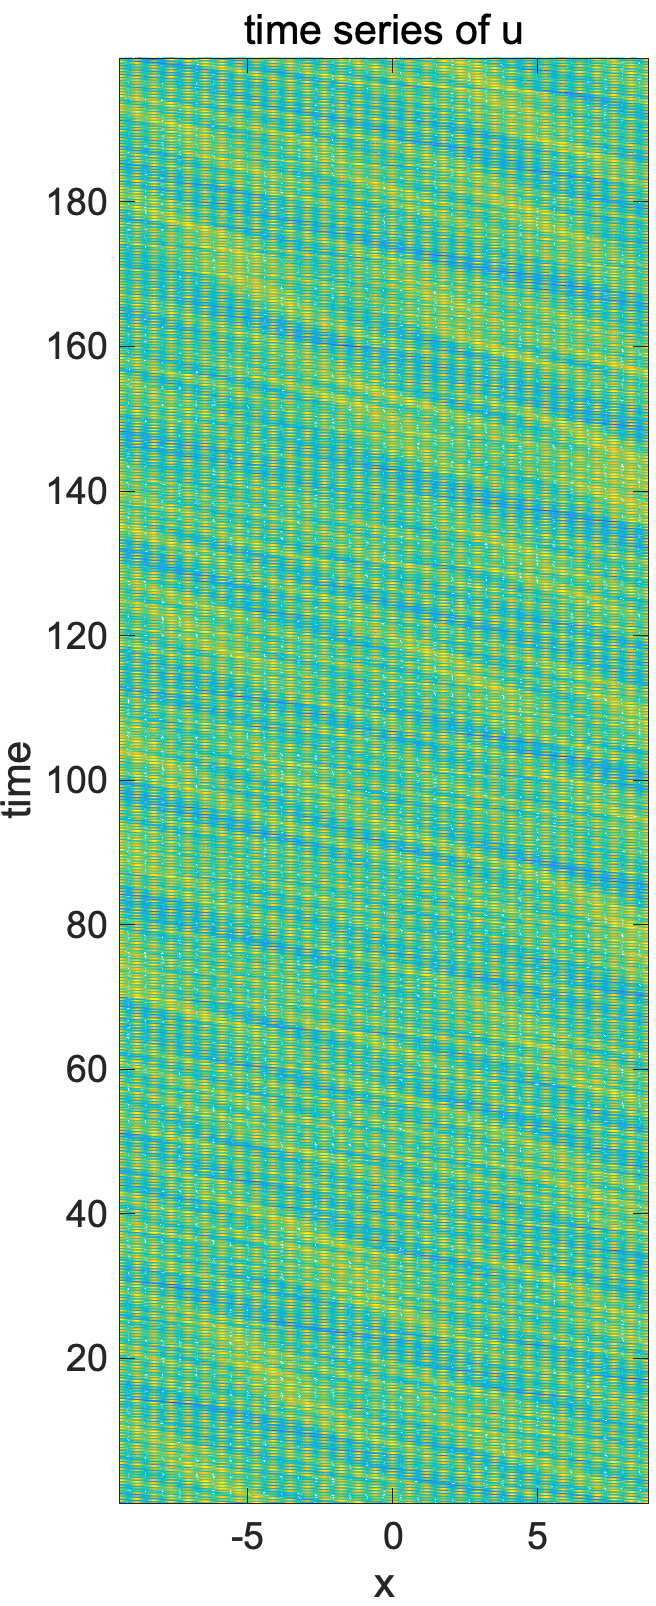
\includegraphics[scale=0.35]{./snap2_J32L3D1E100}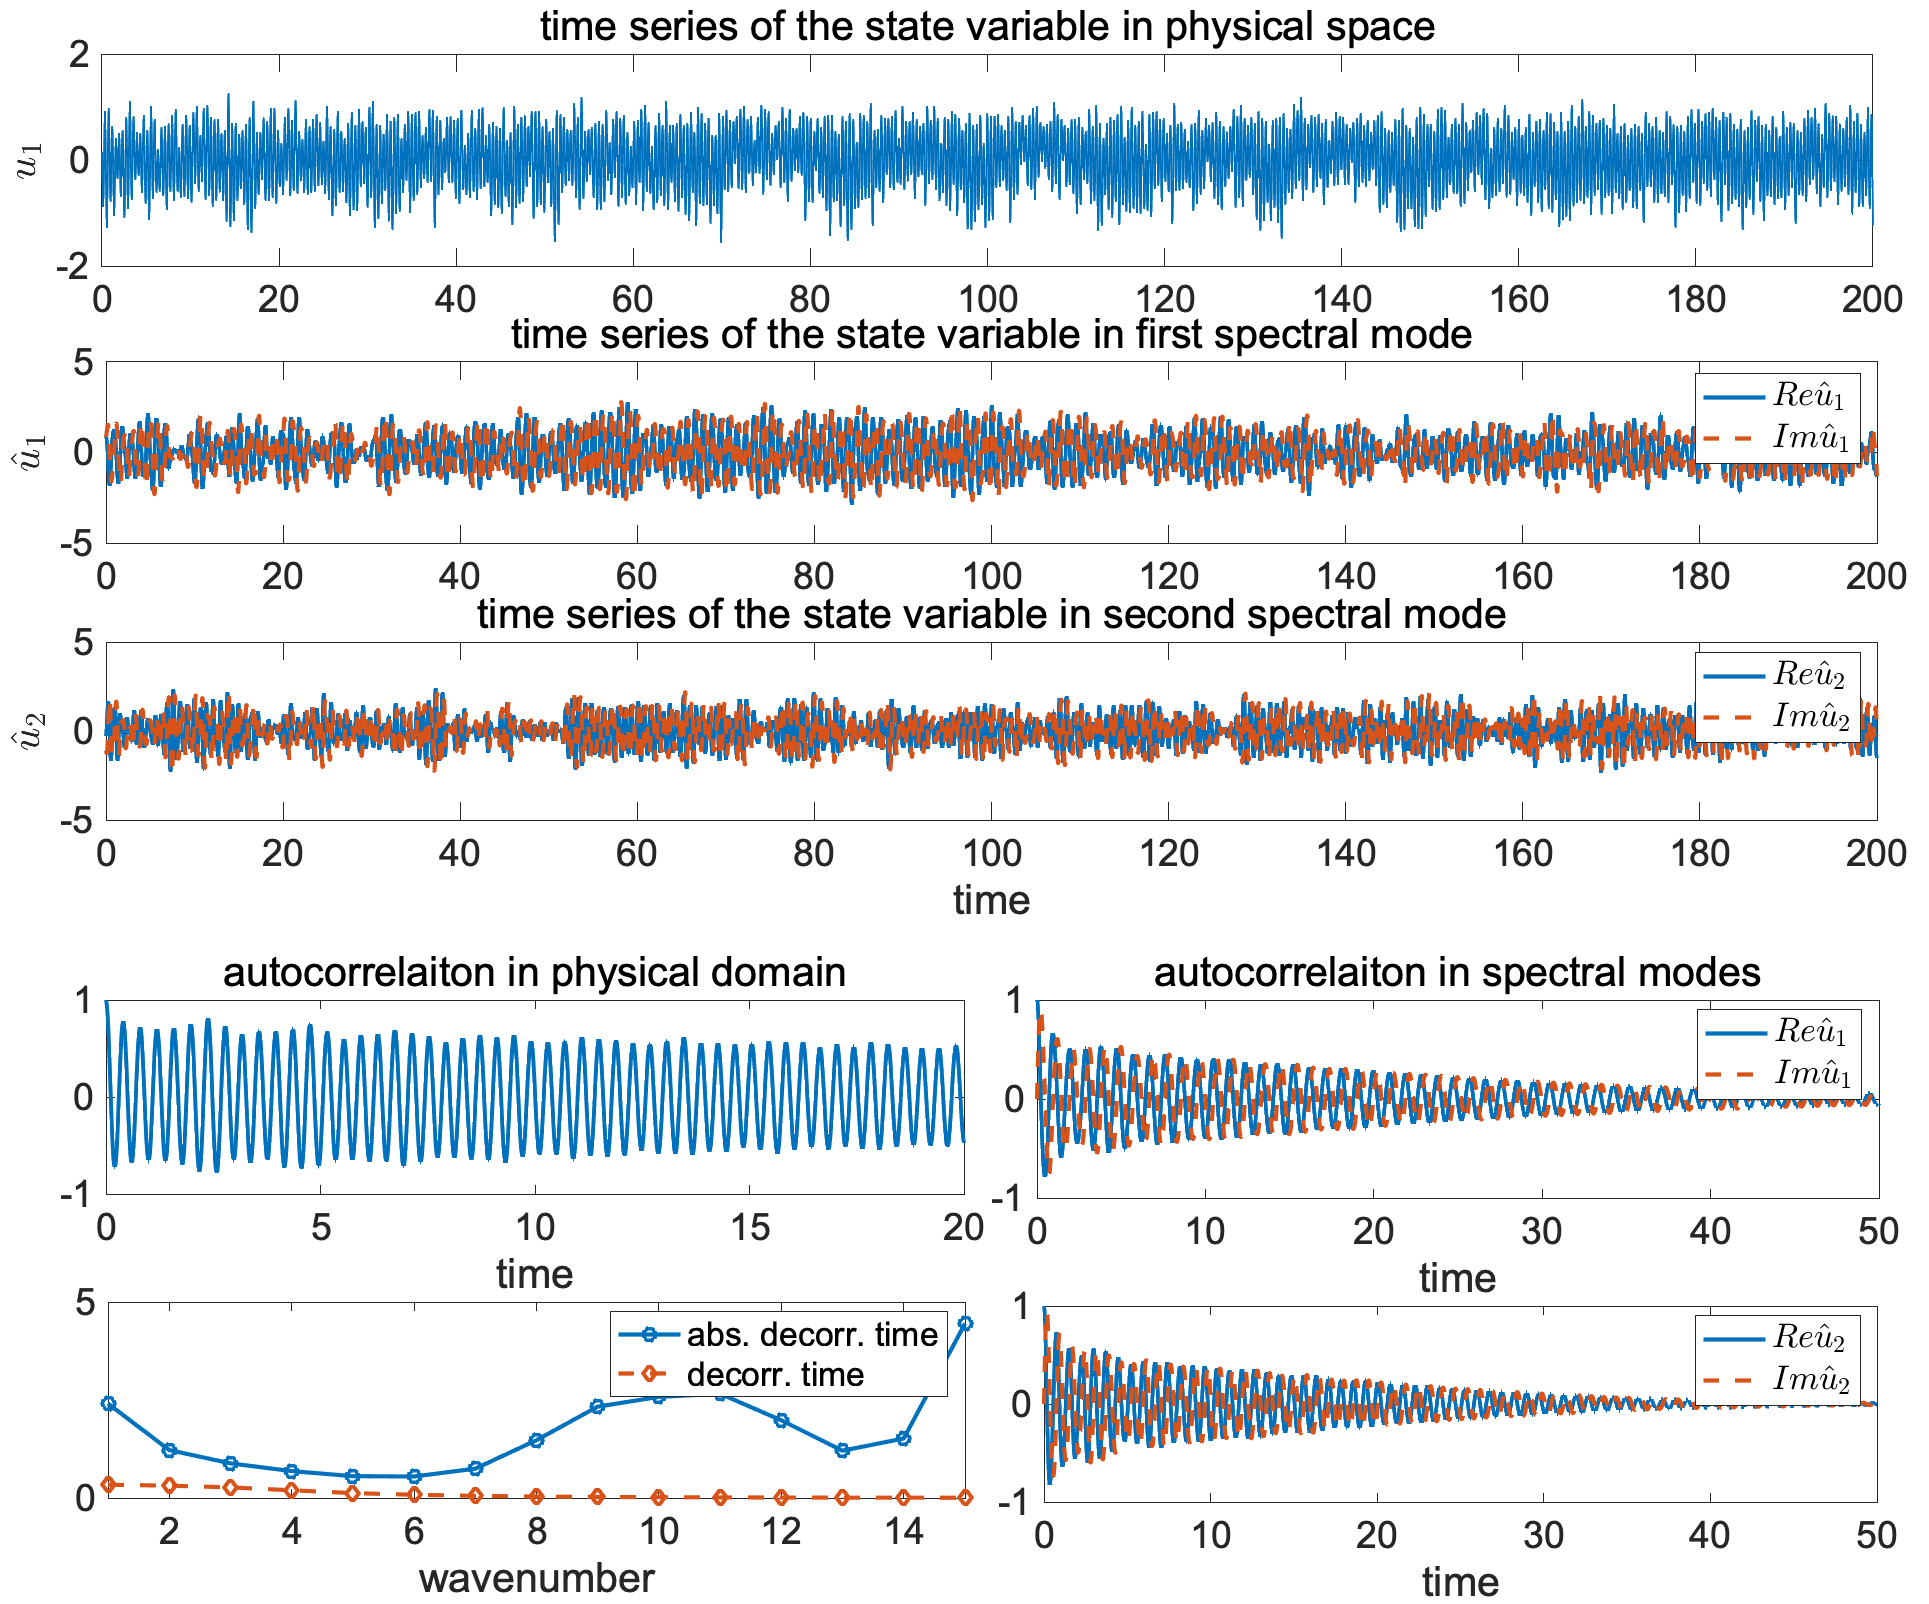
\includegraphics[scale=0.35]{./tseries3_J32L3D1E100}
\par\end{centering}
\caption{Realization of the upstream flow solution with $D_{0}=1$ and initial
state from samples with positive inverse temperature.\label{fig:Realization3}}
\end{figure}
\

\bibliographystyle{plain}
\bibliography{refs_suppl}

\end{document}